\documentclass[ebook,12pt,openany]{memoir} %ebook

%\documentclass[ebook,12pt,openany,onesided]{memoir} %physical book

\usepackage[utf8x]{inputenc}
\usepackage[english]{babel}
\usepackage{url}
\usepackage{graphicx}
\usepackage{imakeidx} % for how to use the index see https://www.sharelatex.com/learn/Indices
\usepackage{hyperref}

\usepackage{afterpage}

\newcommand\blankpage{%
    \null
    \thispagestyle{empty}%
    \addtocounter{page}{-1}%
    \newpage}
\makeindex

\title{Geometron Magic}
\author{Trash Robot}

\begin{document}
\frontmatter
\begin{figure}[htbp]
\centering
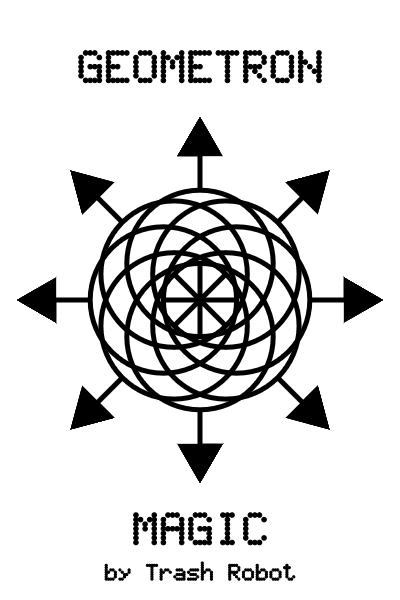
\includegraphics[width=4in]{cover.png}
\end{figure}

\clearpage

\clearpage

\newpage
\thispagestyle{empty}
\mbox{}

\maketitle

\tableofcontents

\listoffigures 

%civilizations
%

\mainmatter

\chapter{Magic}
\hypertarget{home}{%
\subsection{\texorpdfstring{\href{scrolls/home}{HOME}}{HOME}}\label{home}}

\hypertarget{magic}{%
\section{MAGIC}\label{magic}}

Our aim is to share technology which makes all of the elements of a good
life free for all people everywhere. The technology we need to do this
exists. From cheap local renewable energy to dense growth of food to
safe disposal of waste, we have all the material elements of a life of
plenty created by our shared knowledge. And yet we live lives constantly
hounded by scarcity based on activities which are in the process of
killing us all. Why? What is missing from our collective lives? This
work is an attempt to answer these questions and to provide a path
forward using new ways of engaging with existing technology to build the
social structures needed to get from a path of destruction and scarcity
to one of creation and plenty.

Our current model of how we think of technology and ``the economy'' is
based on production and consumption. In the modern world, material is
extracted from the Earth, is processed into ``products'', which
eventually turn into waste, and then the process repeats. This process
will always produce scarcity, as everyone must compete for the limited
resources. That scarcity is managed by people claiming ownership over
the land from which resources are extracted, ownership of the machines
which produce products, and control of the workers making the things.

We cannot continue with this model because in a finite world it will
always consume all resources and destroy all life. We should not
continue because it inflicts misery and fear on all but the small group
of people who own and/or control the system.

Furthermore, even things which are not based on this model, like writing
books or software which can freely replicate on existing hardware, are
forced to conform to the basic logic of this model. While money no
longer literally represents metal dug up from the ground, the
\emph{metaphor} of money is still based on that. No matter what anyone
does, we all need money in our existing system to survive. Under the
existing system if a group of people with no money all want to build a
thing, they can't do it without someone with money-creation authority
blessing the activity. People can physically do it in theory, but as
long as the material needs of survival are controlled by people who
demand money for those things no one but the rich can afford the luxury
of doing useful things for which there is no monetary incentive. This
means that the more people in society produce things which \emph{don't}
require digging things up or doing manual labor, the larger the gap will
be between the money production process and actual creation of value.
This is the reason inequality will always get worse as the information
economy grows. Everyone in the information economy is making money from
replication, while the old economy still runs on production. The more
powerful information technology becomes, the larger this gap will
become, and the rate of increase will keep accelerating.

What we need to recognize in order to move beyond this system is that we
must transition from a consumer society to a replication society, and to
change our value system to reflect that. In the last 300 years we have
dug up a staggering quantity and diversity of material. None of what we
have dug up to build our shared global industrial civilization in the
last few centuries is really ``thrown away''. It's all still here, and
generally way more of it than we want. Some of it is in landfills, some
of it is in wasteful machines that have no reason to exist other than to
keep ``the economy'' going, and some of it is in poisoned water and
soil, but all of it is still around us in some way.

The laws of physics and chemistry will allow us to re-use all these
elements indefinitely just as natural ecosystems have with simpler
elements for the duration of life on Earth. We can in some sense think
of all the trash, toxic waste and useless junk we have created as the
``hardware'' on which we want to create the ``software'' of a just and
sustainable future. In this model, value comes from the power of
replication, rather than production.

In a consumer society, every producer is in competition with every other
producer. In a replication society, creators benefit from replication.
This creates an incentive system for creators which is the opposite of
the existing one. If I find a way to extract a poison from a river using
simple and readily available materials and transform it into a usable
material for building things, it is in my best interest for that to
replicate. I want other people to copy it because only then will
\emph{all} the water get cleaned up. I want other people to copy it
because the more people copy it the more people will improve upon it,
and I will end up with a vastly superior technology to the one I started
with, making the river I live on cleaner than would have been possible
without the broader community of creators.

Replication societies are nothing new. They are much older than the
production model. Any indigenous society which lives in equilibrium with
its environment is replication based. When people living in a forest use
a tree to make a boat to hunt an animal, that is a replication economy.
They use culture to replicate the boat-making process, and stewardship
of the forest to make sure there are always more trees and animals. The
old boats rot and turn into soil which gets turned back into trees, they
teach their children to pass along the system after they die and turn
back into soil themselves, and the system replicates. What we propose
here is to take this older and proven social model used by indigenous
civilizations and apply it to the materials and principles of modern
machines.

So how do we do this? If all the science needed to build a replication
based civilization exists, why are we not doing it now? To build this
world we must recognize what the hard part is about this. It's not
building the things, we know how to do that. It's not organizing people
to do things, we also know how to do that. It's the replication of the
\emph{desire} to replicate a thing. That is what we call ``magic'' for
the purpose of this work. We use this term because no other term fully
expresses the mystery of the process by which we acquire the desire to
do a thing.

Under the current system, desire to replicate plays a minimal or hidden
role. Most people work for money out of fear, create the systems to do
that out of greed, and consume based on being controlled by a media
which exists for the sole purpose of stimulating consumption. All these
processes are separated from one another. We produce at a ``job'' and
consume separately. Anyone not producing or consuming using money is
treated as a burden on the system.

But if we want technology to replicate freely, we need to harness that
spark which causes a person to suddenly feel a desire to create and
share a new thing. That spark cannot be reduced to rules and numbers and
laws of physics. It is the spark that makes us human, which gives us
free will or the human spirit or soul.

Every single technology we use today relies on this magic. Every
computer, every jet airplane, every factory and medicine--all these
things began with some spark in an actual human which was passed on to
other humans. Technology producers today have mechanistic models for
their technology which ignore life. We use the provocative term
``magic'' to re-center all our thoughts about technology on life itself,
starting with the human spirit and going out to the living world around
us. Life is self-replicating and we identify this word ``magic'' with
all living things. We reject any model for our world which is not
centered on the magic of life itself.

So where does this leave us? We want to transition back to a replication
society while retaining the most useful modern technologies. We are
currently trapped in a system based on scarcity that no one can leave.
So how do we get from one to the other? We must first recognize that the
most powerful engine of change in modern society is social networking.
Working alone, any technology we create is of almost no use. Everything
we create requires that we find ways to collaborate and find people to
share with. The core technology which structures all other technology is
how we communicate with one another in complex networks. If we want to
build a radically different world, we must therefore build a radically
different social network. This work represents the creation of a social
network for the sole purpose of empowering this replication economy.

The transition from a consumer to replication society means replacing
the ``means of production'' with the ``means of replication'' as the
fundamental element of our model of society. Of course we will still
have machines that build more machines and people operating those
machines just as we do today. But we recognize that the most fundamental
thing is not those machines but the social network which tells others
how to build those machines and more importantly \emph{why} they should
build those machines. This transmission of the ``why'' is what makes the
process require our use of the term ``magic''.

In order for this to work we need to have media which supports
self-replicating documents which tell us how to replicate technology,
and this media itself must be self-replicating. This means the media
must carry on it documents which in addition to copying freely from one
device to the next must tell people how to copy the actual physical
devices.

Once this process gains momentum we can use it as the basis of a whole
new economy which allows us to progress into a full replication system.
However, initially we are back to the problem of trying to survive
without money in a system which literally won't let us live without it.
Our way out of this is with a middle path in which we build social media
on hardware which can be bought cheaply and given away to the community
as a free resource for very little money and with no material input from
any central entity like a company. In order for this to scale, each time
someone copies the system it must provide more value added up in
monetary units than it costs to build the copy, including the labor to
put it together.

This is much easier than it sounds. Social media today is a centralized
form of power which generates trillions of dollars in commerce, all
based on software. That software has its replication deliberately
crippled by intellectual property so that a very small group of digital
landlords can take money from everyone else in the system. They get away
with this because of the very real value created by linking us all up
with one another in complex ways. From ride sharing to finding friends
to selling and buying things, all commerce can be dramatically enhanced
by social networking. If it costs under 1000 dollars to build out a
local social network of free book-like documents for a community, all we
need is for that to provide 1000 dollars of value and it will replicate.
In even a small and poor community this is an infinitesimal fraction of
the available commerce which can be amplified by social media.

We do not aim to build a ``new social media platform''. We aim to build
hundreds of millions of truly independent social media platforms, all of
which simply replicate documents from one to another, and all of which
exist for the primary purpose of building out the replication economy
which will transition us off of consumption.

To do this in the long run we will rebuild the hardware from the ground
up along the principles of Geometron laid out here. But we can't get
there until we have a network which is financially self-sustaining in
the existing system. At its core this means finding a way to harness the
``magic'', the core spark which makes a person want to engage with a
thing.

Geometron is a way of thinking about technology in which we think of all
technology as a geometric construction. Shaping metal into machines is a
geometric construction. Displaying symbols on a screen or on paper is a
geometric construction. Printing electronic circuits on a board or chip
is a geometric construction. All the symbols we use to communicate with
one another are geometric constructions. In Geometron we rethink how we
program and control machines based on this idea that geometric
constructions are more fundamental than those using numbers. Numbers are
useful tools, but we choose as a matter of values to always place them
in a subordinate role to geometry.

This is the origin of the term ``Geometron'': ``geometry'' combined with
the ``-tron'' ending which is associated with machines. The work here
demonstrates using this method of geometric programming to create a wide
variety of useful things. We replace ``computer programs'' made up of
numbers, algebra and broken English with geometric constructions
represented with geometric symbols.

This book is therefore combining ``Geometron'' with ``magic'' by
building social media based on these ideas about self-replicating media
and geometric thinking, together in a combined whole. The previous book
of Geometron was more technical and also less action oriented. This work
intends to both tell you why we need to build this system and very
specifically how you can immediately engage by copying parts of it and
recruiting other people to copy more of it. We are asking readers to
\emph{participate} actively through direct action. We are asking you to
tell people about this, to share these ideas and build on them. We are
asking you to help us build a world of abundance from the bottom up
through direction action.

Finally, we must address the problematic connotations of the word
``magic'' and why we choose to use it anyway. Many people of many
religious beliefs either view ``magic'' as a word referring to the
``superstition'' of other people's beliefs or some literal power in the
physical world outside of the realm of science. In this work we are
using the word to refer to an observable phenomenon in the world which
everyone agrees happens, and which applies to everyone's religious,
spiritual, or philosophical beliefs. Every belief, be it one called
``religion'', ``philosophy'', ``ideology'', or ``science'', is based on
this replication from person to person. Beliefs are held by mortal
people. We all die. Our minds decay. We forget. What brings beliefs of
\emph{all} kinds to life is their replication. And this is never just
the mechanical process of printing or broadcasting media or preaching in
person. It is the process that happens deep inside us in which each of
us shifts our internal reality, our internal \emph{desires} in a way
which accommodates the new belief system. This can and does happen with
everything we believe. While one person might not believe in the god of
another, none of us should deny the basic observable phenomenon by which
the other person's belief replicated to get to the point that they
believed it. We can call that replication a ``magic'' without
attributing to it any supernatural connotation.

We hope that people of all faiths can use this framework in a productive
way to build new ways of life. Geometron and Trash Magic are not
religious systems. They are systems of organizing information and
materials which can be fit into any existing religion. In order for this
movement to work we must find ways to be compatible with all existing
faiths, and not to attempt to convert to some new faith. Just as we find
all faiths using oil and mine based supply chains today, and
communicating their faiths via the Internet, we will build a world where
all those people are able to carry on their lives in a post-extraction
framework without creating contradictions with the other parts of their
cosmology separate from the mines and pipelines we seek to replace. This
does not make Geometron and Trash Magic ``non religious'' or
``religious'', but occupying a different space in the human mind and
experience and being boosted by the replication of what is already being
replicated. We must therefore build many ``magics'' which are compatible
with all existing human belief systems, and which can replicate along
with them in their institutions.

\chapter{Trash Magic}

Trash Magic is a mode of existence in which we can replicate everything
we need to live a good life locally using the waste streams of the
existing consumer system. We are using the word ``magic'' as in the rest
of this work to refer to the replication of the desire to replicate
things made from trash.

Full Trash Magic is the ultimate objective of all this work. Under full
trash magic, all people, everywhere in the world, can get food, shelter,
medicine, media, sanitation, water, heating and cooling, and the
machines to produce all these for free locally. We will abolish all
mining, all oil and gas extraction and all global physical supply
chains.

In order to achieve this objective we begin small, with something that
immediately provides value, and scale up based on replication of the
thing which provides value. If we can do even the simplest thing which
just barely provides a small amount of value from trash but
\emph{replicates} and \emph{evolves} with intent, we can then simply
guide that evolution and growth to navigate to the complete system as we
engage more and more people with more and more specialized skills and
resources.

To start all this, we turn to the industrial revolution as a guide. Much
of what powered the industrial revolution was using new energy sources
in the form of coal and steam to build machines which build other
machines. Also, textiles have always played a central role in technology
replication, as their products become central to people's culture, which
replicates and brings the textile production machines along with them.

In analogy to all this, we want to build the smallest possible factory,
which we call a Trash Factory, which mimics this pattern but without
mining. We want to build machines that can build machines, or a machine
shop, powered by the local forces of the Sun, wind, and flowing water. A
machine shop is a collection of tools which can work metal into the
forms needed to make more machines. Machine shops are how metal machines
traditionally replicate themselves. We need to be able to melt metal
waste into metal ingots then process that into bars, sheets, rods, wires
and blocks. Then we need milling machines, lathes and drill presses to
machine them into desired shapes. We need the tools of sheet metal work
like the brake and bender. We need an arc welder, torches and some other
basic tools for soldering, welding and brazing. All this must be made
from trash.

Building a machine shop can be based to a large extent on junk cars.
Cars have plenty of steel, plenty of parts to salvage without any
melting or casting, and electrical tools which can be used for motors
and so on. As much as possible we will use things as we find them
without reprocessing. If we can, we'll just get donated old stuff that
is broken and fix it. The machine shop maintained by people good at
fixing broken stuff is as old as the industrial revolution, we just aim
to build this into the rest of our self-replicating media system.

The machine shop also needs to have tools for working plastics, with
molding on metal molds created using the metal shop, and plastic welding
and rework tools. An electrical shop is needed for electric motors and
generators.

A fully functioning machine shop which is optimized to build more
machines from junk cars can be a self-replicating and self-sustaining
factory just by selling machines. We can sell drill presses, milling
machines and the like for money which can support the people who build
and maintain the system.

In addition to the machines which replicate themselves, we will build
all the tools for creating trash-based clothes on site. We will build or
fix broken sewing machines, and use them to create fashionable and
functional original clothing of all kids for all people for free to
those in the most need. If our story replicates as we hope it does, and
people believe in our mission, we should be able to support all the work
to build the system, to operate it, and to deliver the free clothes to
those in need by selling high end fashion to those who can afford it.
All clothes are made on site with waste clothing donated from those in
physical proximity to the Trash Factory.

All the motive power for Trash Factories is provided by one of three
main sources: heat engines, water drive, and wind. An essential
technology which must be integrated into the first generation of Trash
Factory is the trash-built Stirling Engine. This is a very simple heat
engine developed in the 1800s and used widely ever since which can turn
heat into mechanical motion by compressing and decompressing a gas in a
sealed chamber with a piston. These engines have been overshadowed by
the internal combustion engine or the giant steam turbines used in large
scale commercial power plants, but they work well and are well
understood and simple. The primary means of driving a heat engine in
Trash Magic(without setting things on fire) is using the energy of the
sun focused via mirrors onto a heat absorber. Large arrays of mirrors
can be built from trash which track the sun and maintain the focus of
the sun over a large area onto the absorber. The other robotics
technology that is part of Geometron can be used to steer the mirrors as
the angle of the sun changes. Stirling engines can also be run
backwards, creating a heat pump when the shaft is turned. This means
they can be used to cool things, being the basis of solar-powered air
conditioning and solar-powered refrigeration. Solar powered air
conditioners sound almost too good to be true, but this has been
demonstrated well over 100 years ago, it is just not used today for
economic and social reasons. The heat engines are also a very good
commercial product which can be sold(as an off-grid power source) for
money to support the rest of Factory operations.

Water and wind are both pretty traditional: we simply build rotors for
both from trash and source the drive trains and generators from trash.
Water can be waves, tide or streams/rivers/creeks. In all cases, we
envision a factory which has between 1 and 5 people operating it at a
time using between 1 kW and 100 kW.

The absolute maximum available solar power in direct sunlight on a clear
day is about 1 kW per square meter so at 100\% efficiency(which will
never happen) this is up to about a 100 square meters. If we imagine
getting a pessimistic 10\% efficiency, that's up to 1000 square meters,
which is about 30 meters on a side or about 100 feet on a side
square(about a quarter acre or 0.1 hectares).

A reasonable site for a Trash Factory will be about 1 acre, or about
4000 square meters or 0.4 hectares. This will be enough space for a
machine shop, the power station, and the various staging areas we need
for incoming waste streams and outgoing product streams. When possible
we site near flowing natural water and use extra power to both pump
water uphill and to clean it up for drinking. Water can then be both
used to drink and used to get energy back out as it flows downhill from
a water tower or hill top reservoir. Our goal is to be a very
scaled-down version of the River Rouge factory from the Ford Motor
Company from the early 20th century, where a constant flow of raw
trash(instead of raw material from a mine) comes in one side and a flow
of finished manufactured goods flows out the other side.

The Trash Factory can be sited based on convenience to resources, cheap
land zoned for heavy industrial activity, and easy access. It does not
have to be an ideal retail location. The retail side of the Trash
Factory is free stores and existing shops. We can make things to
directly provide for free for those who want, providing warmth and
protection with fashionable and well-fit clothes sourced from local
trash while also sourcing products for local stores shelves we sell for
money to support the Factory. This also applies to all the machines
produced in the machine shop: we can sell welders at a welding shop,
heat pumps through an HVAC(heating, ventilation, and air conditioning)
distributor, drill presses and machine tools to auto shops, etc. Also,
providing a mix of free and commercial products to our local community
creates the human relationships we need to establish to keep our supply
chain flowing of trash we get for free from existing waste streams.

Again, the Trash Factory aims to always produce more value than it
consumes, both bringing in enough cash to support the people operating
it and the land and also providing material support for whoever is the
most wanting in the local community. Every kilogram of mass we convert
from trash to products locally takes that kilogram of mass out of both
the landfill waste stream and the mine stream of consumer society. If we
can make this replicate and evolve, we can keep removing more and more
energy from that system over time, and pumping more and more energy into
our system. As long as replication of this system takes less energy than
replicating the existing systems we will naturally consume the old
system for reasons of simple thermodynamics.

But where does ``Trash Magic'' fit in with all this? Trash Magic refers
to the transmission of this system of trash-built and trash-sourced
factory using the self-replicating media platform described in this
work. Every machine, article of clothing, every clever hack and
structure of business or organization will be documented in a library of
books(including this one) which are kept on free media and network
infrastructure we build into all of our systems. In the beginning this
will be the Raspberry Pi(a very cheap and open source computer) based
system which starts building our network, along with off the shelf
commercial wireless network infrastructure. As we develop our system it
will evolve into the fully trash-built media described later in this
work.

Full Trash Magic involves taking the Trash Factory system described here
and scaling it up to all things we need. As we grow we always direct all
excess value created by the system into helping the most needy in the
immediate physical community around the Factory. As this pulls more
energy into the system, we will be able to get access to more land and
resources outside the property system. Directing resources to those with
the most needs first will abolish poverty in very localized areas.
Abolition of local poverty will enable more space outside of the
property system to flourish, on which we can create products which are
all outside the property system.

This will ultimately include the whole set. We need to build fresh water
generators from dirty water, and build a toilet infrastructure which
turns human waste into compost which is used to grow things locally
including organic fiber crops for toilet paper(which can also be a
product of the Factory). This waste disposal and composting system will
be integrated into a system of local synthetic biology, where we use
modern biotechnology techniques to control microorganisms and fungi to
make all the medicine we need on site. Again, building bioreactors which
can make all medicine is nothing new, we just need enough human energy
in the system that we can attract the talent in the form of experts who
already know how to build such systems. Our aim initially is not to
invent anything, but to create the social connections which allow people
with expertise to connect with real local community needs and then to
scale that through self-replicating media. If we can make clean water,
machines, clothes, medicine, food, and media on site, we have a system
which can sustain human life without mining or oil as is our goal. You
can think of our whole social media system as like a ride share app but
for finding the people with whom we build a sustainable civilization.

Again, we must reiterate that this is not some futuristic hypothetical
technology. Creating free web pages on free computers which tell you how
to make things from trash is simple. Making things from trash is known.
The waste is plentiful. 300 years of industrial production brings the
whole periodic table of elements right to your doorstep. The needs of
the most impoverished and marginalized people in any given local
community are known. The mass peer-to-peer media network of the Internet
exists which can spread all of this. All we are saying with this work is
that these dots can be connected. The only thing missing is the
\emph{will} to connect these dots. And of course while we might already
have the will to do it, what we need to make it scale is the ability to
create specific detailed plans and replicate the desire to carry those
out. The media platform documented in the rest of this work will allow
us to do this. The revenue we will generate by simply building the free
social network of free books will provide the startup capital(not
financial capital, but resources like land and human attention) to build
our first Factories.

Full Trash Magic can exist on just a few acres with just a few dozen
people. We can achieve this in our lifetimes if we focus on our
objective and work together!

\chapter{The Pibrary}
\hypertarget{home}{%
\subsection{\texorpdfstring{\href{scrolls/home}{HOME}}{HOME}}\label{home}}

\hypertarget{the-pibrary}{%
\section{The Pibrary}\label{the-pibrary}}

The Pibrary is a network of free books distributed using the Raspberry
Pi, a very cheap open source computer designed primarily for educational
use. The goal of the Pibrary is to be an extension of the public library
system into more public spaces and with more free and more local books.

The Pibrary represents a fully free network, meaning everything is free
of copyrights or other intellectual property, everything is available in
a public space for use by whoever wants to use it, and everything can be
freely replicated by other people in other places.

The Pibrary is centered on public spaces, meaning spaces anyone can get
access to without any restrictions such as public parks or public
streets or any other outdoor space which we do not restrict access to
based on money. This can include private property as long as the owners
of the property are willing to create a truly open space which welcomes
all people regardless of social or economic status on a 24/7 basis.

The free computing element of the Pibrary consists of mobile raspberry
pi computers with portable battery and solar panel as a free community
computing resource for use in public spaces by whoever has the greatest
need for free access to information. This is to be an extension of other
mutual aid projects like Food Not Bombs which provide basic goods and
services for free to the most marginalized people in public spaces. The
solar panels and batteries can be used to power or charge mobile
devices, a critical infrastructure need for unhoused or traveling
people. The Raspberry Pis are installed with no private data, no logins,
no passwords, and are intended to be used that way so that they can be
safely shared. The only purpose of the Pi is to access the Internet for
free, just like a free public computer in a public library.

The basic Raspberry Pi mobile terminal setup consists of the Pi board
which is about the size of a deck of cards and costs about \$60, the SD
card the operating system is installed on, a keyboard, a mouse, a small
mobile screen, a 12 volt lead acid battery, and a solar panel and
charger. The whole system costs about \$400 and can all be purchased
online from many vendors. In order to charge devices the kit must also
have a 12 volt USB power hub to break out the battery power for charging
USB devices.

The Raspberry Pi is also used as a home web server for creating, editing
and sharing the self-replicating documents of the Geometron system. To
run a Pi at home we need a lot less infrastructure. The keyboard and
mouse and a standard TV or computer screen can be used once to set it
up, it can be powered off of a wall plug, and then run ``headless'' with
no screen or peripherals, accessed over entirely over the network. This
server can be accessed by people anywhere in the world by using port
forwarding over the home router or router in a public space to connect
it to the outside Internet.

Internet access is provided for free in public spaces by wireless
hotspots with clearly posted log on information. We can beam Internet
into public spaces with directional antennas and wireless network
extenders. All of this physical infrastructure is provided for free by
donors from the local community. It is a public resource.

The primary purpose of all the media hosted on the Pibrary system is to
create a free library of books which contain all the knowledge required
to build a society based on the principles of the last chapter: built
from trash and powered from the sun, wind and water. This will include
science, technology, history, culture, commerce, and any other deep
knowledge about and for a local community. All of these books consist of
collections of documents which replicate freely from one server to
another without any restrictions. Each copy of each book can also be
edited, deleted, or moved around on any server by anyone at any time.

The Pibrary is a network of free self-replicating books. This is not a
network of users. There is no private data, there are no users, no
logins, no passwords, no encryption, and no databases. While we are
creating a vast universe of documents, each Pibrary will have a
collection which is limited based on a focus of immediate interest for a
relatively small community with a shared purpose.

Part of the infrastructure of the Pibrary is domain names for public use
which can host copies of all the documents in our system. All of these
public web pages, like the Raspberry Pi servers, have no private data,
no users, and no databases. Anyone can copy files onto them and off of
them, or delete them at will. Pages can be forked down to make more
libraries with more books and more libraries inside libraries. Whole
forks can be deleted by anyone at any time. Our resilience against
deleting is to constantly copy books to many places again and again. We
are building media which behaves as a living organism, replicating,
dying, and evolving as part of our culture as humans.

The domain names for these public web pages are selected to correspond
to public spaces like streets, parks or bodies of water, with top level
domains other than .com so that they are non commercial and not
personal. Some volunteer from the community can buy the domain and pay
for commercial cloud hosting at some standard web hosting vendor, and
install the system on that server. It generally costs about 10 dollars a
year for the domain and another 10 dollars a month or so for the
hosting. As long as our network is providing significant community
benefit this should be a relatively minor cost to get paid for by a
volunteer.

We create physical flags to display in public spaces which point to the
domains which host the books. These flags are created by sewing solid
rainbow colored felt letters in a block font onto a black cloth
background about 3 feet by 3 feet square. Flags, like everything else,
are meant to be copied widely and displayed publicly. Flags fly in
physical spaces which are represented by domains which host books we
create, edit and replicate using the network of free Raspberry Pi
computers.

Another powerful tool in our network of self-replicating books is
Github. Github is a company which provides free(free for open source and
that includes everything we do) hosting of documents which can be copied
from anywhere on the Web. We can create private instances of Geometron
servers on home personal computers which have local web servers set up
which only run on that machine. These are used to edit local copies of
the whole system including any books we want to save. As these are
replicated and edited, they can be ``pushed'' to Github with Github
Desktop, a GUI app. Using Github to move books around provides a backup
where if servers are all wiped out the data can't be edited without
access to a personal Github account which is based on Github's security.
Also Github has enough bandwidth and protection against surges in
bandwidth that it can be a source for replication to many servers all at
once. Anyone anywhere in the world can copy whole libraries of books
with simple clicks in their web browser to their personal Github
repositories, then push it out to the public and copy from there to any
other server. This network of potentially millions of Github accounts
and millions of Raspberry Pi's and millions of domain names can be
constantly supporting a free flow of replication of books from server to
server across the globe.

The format of ``books'' on the Pibrary is the ``magic book'' described
in the next chapter. This library of free books can form the basis of a
social network which provides the same benefits of modern networking
applications but with direct community control. Books can be created to
document all commerce, organized by the people engaging in that
commerce. The same efficiency improvements which are currently monetized
by Silicon Valley can then be kept in local communities, which brings in
enough wealth to materially support the people building the network. As
the amount of wealth generated by the network increases we will direct
all excess to those in the local community with the most need.

The use of the Network to direct resources to those in the most need is
mutual aid. The network helps people and those people help the network
by representing it in public, sharing the information with as many
people as possible. This applies to everyone. As the network generates
more wealth it should be possible to eliminate poverty in very localized
areas covered by the network. As this happens we can use the network to
build more and more industries up using the Trash Factories and this can
amplify the process. Network value in commercial activity funds
industrial value which funds more network expansion and so on. As the
network grows and we can support more people, those people can solve
harder and harder problems and scale up what we can make in the Trash
Factories more and more. As this knowledge is generated, it will all be
synthesized into more free self-replicating books which are published
onto the Pibrary network. So our manufacturing supports growth of the
network, but the network is also supporting the growth of manufacturing
by replicating all the knowledge required to copy our processes.

The Pibrary creates and enhances public spaces. Selecting the right
physical space to inhabit for this is one of the most important parts of
building a successful network. We need to choose spaces that have the
absolute maximum possible intersection of people. We must ask the
question: if a place is about 10 yards across, what place in a given
area a couple miles across has the widest range of people crossing it in
any given day? Of places like this, what is the most freely accessible?
We must evaluate accessibility based on sidewalks, access by car, access
by public transit, by bike, wheelchair, or any other means of access
relevant to the local community. But we must also consider accessibility
in terms of it being legal to be there, there being adequate restroom
facilities nearby, places to rest or work or sleep, shade or other
shelter, and a generally welcoming culture.

The public space being activated by a Pibrary does not need to always
have a Raspberry Pi or solar panel. It can just have a flag or sign or
markers which point to the domain which has the copies of the books
maintained about that place. It can even be invisible, with a known
domain being used by people about a place without any obvious
infrastructure in that place other than the place itself.

The Raspberry Pi can also serve as a monitor for the environment,
measuring aspects of the water, air, soil, living things and anything
else of interest to the community. In rural areas, sequences of wireless
network repeaters on off-grid power can go along rivers and streams with
local Raspberry Pi's with sensors measuring water properties and
delivering that information via the web to the rest of the network. This
can put the land, life, and water itself onto the network and connect
all of us humans on the network more intimately with these systems.

\chapter{The Magic Books}


The media which drives this network is the Magic Book. The Magic Book is
a format for electronic books which lends itself to easy replication
across the Internet and easy editing. We use the term ``magic'' as in
all other places in this work to mean that people replicate them
themselves. That is, with simply copy/pasting links and clicking on them
in browsers anyone on a network can copy any book from any server to any
other server.

This is not like Google Docs where documents are attached to ``users''
who log into a cloud server controlled by Google. We use cloud hosting
for public-facing web pages, but they are all able to be read by anyone
anywhere in the world freely without any log ins or passwords. And all
these books are created, edited, and shared on the local Pibrary
networks hosted on physical Raspberry Pi based web servers which are
shared freely in our local physical community.

Also, we are using ``book'' as a metaphor. What is a book exactly? How
is it different from other media? A book can be physical or digital, can
be a private document or public. But what distinguishes it from things
like articles or news is that it is self-contained and encapsulates a
large body of knowledge in a coherent whole. A book can evolve over time
and can get re-written but it has a fundamentally different structure
from the news feeds which dominate social media today. Also, we
distinguish these books from wiki's like Wikipedia. Wikis are databases
of articles. These articles are the fundamental element of the whole
thing, and are not organized into book structures. It is hard to write
down a clear definition which distinguishes an article from a book, but
for our purposes a book is a collection of chapters, each of which is a
text document, and all of which add up to some coherent whole.

All books are released by their authors into the Public Domain with no
restrictions whatsoever. We do not use the kind of restricted licenses
favored by Creative Commons or the Free Software Foundation, but
explicitly release books under the Public Domain.

Books, like everything else in the work described here, are
self-replicating sets. That is, collections of things which all
replicate as a set easily by anyone on the network. The main element of
these sets are called scrolls and these are just text documents in the
Markdown format. Markdown is a very simple text format which is used in
a wide range of online content, which in its simplest form is just raw
text, but has a few simple additions like using asterisks for italic,
double asterisks for bold, and number signs for headings. While using a
markup language like this with a little bit of syntax is in some ways
more complex than the completely point-and-click driven editors like
Word or Google Docs, this is designed to make the documents compatible
with pure-text formats, which is important for making them easy to
replicate and edit as we move them freely across our network. We believe
that the usability cost of Markdown is worth it for the usability gain
of being plain human readable text. The Scroll format used in this work
is Markdown converted on-the-fly into HTML using the open source
JavaScript library showdown.js. This allows us to set format parameters
like font, size, color, and how text fits in a screen using standard web
development methods, adapting the same text document to any look and
feel or screen size we want(a huge advantage over pdf). This reliance on
standard web development methods allows us to have our format work well
on all web enabled devices from mobile to tablet to desktop to big
screens and of course our free public Raspberry Pi computers without any
software other than the browser.

While our primary media format is in the web browser, it is also useful
to be able to generate physical bound books, also for free distribution.
There are a number of ways to do this, but the one we recommend and are
using for this work is LaTeX(pronounced LAY-TECH or LAH-TECH, the ``X''
is meant to represent the Greek letter ``Chi''), and document formatting
system developed for the typesetting of technical work. Like Markdown,
this is a human-readable text format in which standard text characters
are used to indicate to the computer how format will work. For example,
while Markdown uses asterisks around a word for italic, LaTeX uses a
backslash command ``\emph" along with curly brackets around whatever
goes in italic. The most important thing about using LaTeX is that for
when we create more technical works diving into the physics, engineering
and math needed to build the world of full Trash Magic that it makes
that easy. This system is already widely used by technology creators and
scientists so while it has a steep learning curve it is useful for the
experts we are inviting into this system to create technical books.
Also, it is compatible with a number of other web-based systems of
technical documentation like the Jupyter Notebooks which are an almost
universal means of communication now in applied sciences where
calculations are done on data using Python or other popular data science
languages like R. Another widely used and open source Javascript
library(Mathjax.js) allows us to optionally turn on this math
typesetting in the Markdown-driven scroll documents as well, so
technical books can be written entirely in the Pibrary format and then
moved to LaTeX with the math formatting staying the same. Conversion
from Markdown to LaTeX can be enabled with Pandoc, the''swiss army
knife" of document formats(see pandoc.org for details). Once a book is
in the LaTeX format it is compiled into .pdf in whatever book size is
appropriate. We generally use this to compile to two formats: the letter
size in the US or A4 in metric countries for printing on standard home
or office printers to bind in three ring binders and the 6x9 inch format
for binding from print-on-demand publishers. We use Lulu Press(lulu.com)
to create the bound copies in various formats.

The exact means by which books are replicated will be discussed
elsewhere, but essentially it is all based on building links to scripts
which can be run from a browser which fetch lists of files and use that
list to fetch all the files. The best way to learn how to do this is by
example, and the replication of this work will involve directly showing
people how to do this in person, via video, and via real time online
communication we will be setting up in the coming months.

So far we have discussed the format of the Magic Books but not the
purpose or what books we will share first. The purpose of the library of
books we are creating here is to be a repository of all the knowledge
needed to build full Trash Magic. This means we need to create a culture
with everything that goes along with that: history, philosophy,
politics, technology, science, math, and all the wisdom required to be
stewards of the land we are a part of. This system of books also needs
to self-support. This means that as a social media platform it needs to
generate economic value measured initially in money which can provide
material support to those of us creating and replicating the network.

The beginning of this library is the books created by the author of this
book, Trash Robot. This includes the Trash Magic Manifesto, the Trash
Magic Action Coloring Book, and the first Book of Geometron, as well as
this book, Geometron Magic. Trash Robot is also in the process of
creating another book, Trash Physics, which is part memoir, part
criticism of the structure of modern physics, and partly the start of a
whole library of physics texts based on the principles here.

The way the library of Magic Books we describe here will become
self-sustaining is by documenting the commerce in local communities in a
deep and organized way that no existing resource does. This is not just
a business directory. It is the creation of a new level of social
networking in physically local spaces that does not exist on today's
Internet. We will work with local people to create books on local
history, local culture, the local economy, the local government, local
mutual aid and outreach organizations, local libraries, local religious
institutions, and compile all of into books which are shared on our
system. Again, this is not a wiki covering existing things. This is a
library, creating new deeper connections than exist today, diving deeper
into history and culture than the existing Web does. It is also not
news. We aim to create new social links in physically local spaces with
our system which enable people to engage in new commerce with each other
locally. We call these books the Books of the Street, where the
``street'' here refers to a local public space where we site the Pibrary
discussed in the previous chapter.

The Books of the Street are doing more than documenting existing
networks and businesses and people. They are \emph{creating} social
networks of actual humans in a physical space which do not exist in
today's globalized world of cars, planes, and long distance
communications. They represent a cultural shift to extreme localization
of communities localized to just a couple of miles across, which still
maintain the flow of global information across the entire human race.

Creating connections between people which did not exist before can
enable commerce. Enabling commerce creates cash flow in exactly the same
way it does in centralized commercial social media. This cash flow
generated by the network creates a strong incentive for network
participants to materially support network creators. Supporting us, the
network creators, allows us to spread the network, and if that spread
generates more value wherever it goes, that becomes self-sustaining in
growth. Initially, this network is simply a social media platform which
provides a totally free, non-capitalist (no money, no property) resource
to those in the existing capitalist economy. If we can scale with
positive cash flow in each local node, this creates a much more
efficient scaling mechanism than existing venture capital backed
technology startup companies, which generally scale at a loss in order
to gain market dominance. Without the billions of dollars of venture
capital money required to scale, we can move faster and be more
adaptable than those networks, enabling us to ultimately take away all
their market share bit by bit from a bottom-up approach.

Consider any ``technology'' company today which makes its money on
creating links between people. From ride share to dating to advertising,
all these companies are simply connectors. They connect people with
other people and then demand rent from us for doing so. A free network
driven locally from the bottom up with community owned hardware and no
intellectual property can easily defeat this network one street corner
at a time. We can take Silicon Valley down to zero if we can get the
right growth model of our network, and it is in the best interest of all
people that this happen as soon as possible, since the predatory model
of Silicon Valley is destroying us all. We are asking people with great
urgency to contribute to this campaign.

A final note on what books we choose to replicate on any given Pibrary.
In a traditional library, more is always considered to be better. The
more resources a library has the more books they buy, and it is assumed
that readers use search and browsing to find what they need with no core
specific purpose. This is not the case of the Pibrary. The Pibrary has a
purpose, our purpose is to create self-replicating media which can
transmit self-replicating technology made from trash which can provide
for all human needs for free. We therefore are very specifically
\emph{not} trying to just add more and more books. We want the selection
of books to be very aggressively curated by the caretakers of the
Network to specifically carry out whatever the next task is in any given
community to bring all of humanity closer to full Trash Magic. In some
cases, this might mean an individual person carries an individual
Raspberry Pi with just one or two books, specifically fro the exactly
actions of mutual aid and direct action in which we are engaged.

\chapter{The People of the Network}
\hypertarget{home}{%
\subsection{\texorpdfstring{\href{scrolls/home}{HOME}}{HOME}}\label{home}}

\hypertarget{people}{%
\section{People}\label{people}}

The heart of a network of people is the \emph{people}, not the
technology which connects us. We aim to build a network which can
materially support creators on the network. To do this we must make the
network provide so much more benefit to participants than the cost of
adding physical infrastructure and providing support to the creators
that people will do so out of self-interest.

We aim to build a network which helps as many people as much as
possible. We aim to start by helping the most marginalized people with
direct assistance in the form of communication, knowledge and power
resources. From there we aim to connect all the other people who share
physical space in local communities.

Big Tech doesn't care about anyone's community. They provide just enough
increases in efficiency and human connection between people to get us
addicted to their products, then extract all excess value that they can
using the power of monopolies to create a vast suction of value from
everyone everywhere in the world to the professionals of their industry.

Multiplied by hundreds of millions of communities, this leaves trillions
of dollars on the table in commerce which can be recaptured by local
communities away from Big Tech. If we can provide more increases in
efficiency and more human connection than Big Tech but keep the value in
our local communities, we should be able to take every single dollar out
of their system, to totally destroy Silicon Valley. Our long term aim is
to purge the Earth of them, to totally destroy the culture and society
of the so-called ``tech industry''. We should be able to engage in
commerce anywhere in the world without sending a single dollar to
California.

This all starts with the simple act of creating networks of people
dedicated to the shared goal of building out this network.

The physical machines and digital files which make up the technology
system are released by the creators of the network from the property
system in order to make replication more free.

This chapter is a recruitment request. We are looking for all these
people to join us, to join this movement and this network. We need you
to collaborate to share knowledge and resources to help build this.
Ultimately we want this network to belong to everyone everywhere, but
right now we are directly asking all the people below to reach out and
collaborate to immediately bring this network into being in the physical
world.

\textbf{The people of the network.} We create this network to support
ourselves. We believe that building and releasing for free these
resources can create enough value for enough people that they will
support us directly to keep freely creating and sharing. It is my
intention to live this way as soon as possible, to get food, shelter,
medicine, transport, technical resources, and places to work provided by
people who benefit greatly from the expansion of the network. This will
start out as a very hard thing, supported by a few large donors and many
small donors, and will become easy as we get network scale effects. The
author will become a person of the network as soon as I possibly can.

\textbf{Public Librarians.} The Pibrary is an extension of the library
system. The public library mission is make knowledge as free as
possible. The pibrary consists of freely created, edited and shared
documents on free hardware maintained in public spaces and available to
all. Public libraries currently serve as a computing and Internet
resource for people with no other access. The Pibrary brings physical
computers out to the streets with 24/7 access, taking some load off of
the computing resources in the physical library, and extending hours and
accessibility of the resource. By being useful for other communities,
the Pibrary can be self-supporting, extending the reach and impact of
the library without costing money from the base library budget.
Pibraries also extend the effective collection of the library, as
user-generated content is all completely free and openly shared,
replicated globally from one to another potentially over billions of
servers. As we scale up, it should be possible for a local public
library with almost no budget or resources to have access to a very
large collection of free titles. Libraries with maker spaces already
have STEM education curriculum and often already have Raspberry pi's,
and this network simply adds to the impact of that, adding content to
it.

\textbf{Authors.} If you are someone who writes for the common good of
humanity who believes in free knowledge without the limits of
intellectual property, the Pibrary can be a platform for creating
explicitly free work. As we scale, the intent of this network is to have
authors created through direct material support from the communities we
serve. If we can get authors generating knowledge to provide all the
good things in life, this will be a self-sustaining system without
money. In the short term, it can sustain authors via driving traffic to
voluntary support pages like Patreon or links to buy physical copies of
books with a profit built in from self-publishing platforms like Lulu
press. No work may be posted unless you relinquish all copyright to
public domain. No exceptions.

\textbf{Unhoused people.} This is a mutual aid based network. This means
primarily that we are providing fully free infrastructure and services
in public spaces on the streets, directly controlled by the people who
need it. This means we will provide free wifi hotspots, free solar
powered device chargers, and free easily portable physical computers you
can use 24/7. It also means that we will be co-creating documents which
have all the resources available in the local community including
contact information for aid organizations, jobs, housing resources, harm
reduction organizations, and anyone else who is providing resources. It
also means we are going to be asking for your help in sharing and
growing the network. If our network grows we will eventually be able to
make all the things of a good life free for all people, and the only way
to do that is to provide for those who have the least first. And the way
to do that is to incorporate you directly into our emerging community,
where you can actively engage and contribute by sharing your own stories
and creations with the other readers and creators on the Pibrary
network.

\textbf{Teachers.} This system can be used by writing teachers to help
students co-create published books directly to their local community as
an alternative to papers read only by the teacher. It can also be used
by anyone teaching people how to code as a development environment which
can be run in a web browser, then published to the network and shared
with the world instantly without any gate keepers. Rather than learning
how to code in a job for a company, we teach people to code by directly
building web content immediately and publishing to the network for other
people to build on. Our aim is to transition all teaching from job
training to direct creation of useful resources for people's
communities. The Raspberry Pi can save a lot of money as a low cost
powerful computing resource, and the more people we share this with the
better.

\textbf{Traveling kids/dirty kids/crust punks.} Think of the Pibrary as
a deep sign, or perhaps ``hypersign''. A cardboard sign, cloth flag with
url or QR code can point to a web-based mirror of the chaos books. These
books can have \emph{anything} on them. You can share your stories,
share whatever you have to share, to sell, etc. By forming connections
with other people who maintain the networks and are supportive, you can
maintain documents for free online with no gate keepers, no censors, no
algorithms, no passwords or logins, just free things to share freely
which can help get the information out there that you need to get the
aid you need to stay happy and healthy on the road. You have a critical
role to play in growing the network, sharing our resources and story
with the world. This is a knowledge network, a linking of people who
inhabit shared physical spaces. You can help us to link up all the
social networks which connect in physical crossroads like downtowns and
truck stops across the world. And we can help you by helping to promote
direct mutual aid to help you on the road. In a world without property,
you are also the pumping blood of our network, moving physical goods to
place to place without money.

\textbf{Scientists, mathematicians, academics.} This is a publication
platform with no barrier to entry. If you produce knowledge you are
willing to share freely with humanity, this can be a platform which not
only shares what you have created but which is built in such a way that
others can immediately build on it. You can write a totally incomplete
paper with most of the important parts missing, and if it gets to the
correct collaborators, they can build on it and replicate it back to the
network and you'll get back something much better than what you started
with. This is a new way of doing research, where we do not associate
documents with individual people but with a process of improvement where
all readers and writers are co-creating the work over time. We advocate
letting go of ego and prioritizing progress over personal accolades.
However, this publication is still compatible with career boosting
publications as it can be treated like free online archives are now with
preprints of articles that eventually go into gate kept peer review
journals. These documents are compatible with the LaTeX system of
mathematical type setting, a small modification is all that is required
to turn it on(documented here).

\textbf{Keepers of indigenous knowledge.} We aim with this knowledge
network to bring back a more dynamic living type of knowledge that has
existed throughout the world in indigenous cultures for thousands of
years. It is our hope that by bringing free computers, free Internet and
free off grid power for it all to communities with posses indigenous
knowledge that those people will be empowered to share using this
platform, both with each other and with the world. Our network is a
hybrid of oral tradition and digital methods, where community members
are all co-creating documents which are then passed along freely to the
whole of the community. The world today is in desperate urgent need of
indigenous science and technology if we are to restore equilibrium
between humanity and the living world. We need the traditional
technology and culture to be able to blend with that of the Internet and
computers if we are to navigate the whole of humanity out of our current
predicament. Our intent is to get the hardware into your communities,
teach your teachers, elders, and other stake holders how to run and grow
the system, and then it becomes your network to shape as you see fit. We
also aim to have the network of off-grid computers and wireless links
connect with environmental sensors, putting the living Earth onto the
indigenous network in a very literal way, hopefully giving it more of a
voice in the affairs of the our world as well.

\textbf{Mutual aid workers, harm reduction, street outreach, community
organizers.} The pibrary should have a book dedicated to community
resources. This can be a directory of links to resources, people,
places, organizations, jobs, housing, really anything that is freely
available to help people out should get cataloged here and that should
be actively maintained by all. Think of this like a phone book for
resources for those most in need of those resources(any resources).

\textbf{People who have too many physical books.} You know who you are.
You know more than half your books are ones you'll never look at again
and don't need but both are not sure which half that is, can't bear the
thought of them going into a dumpster due to a library donation drive
getting too many books and don't want to lug them all over the place.
What you really want is to get them into the hands of an actual reader
who will actually read them. The pibrary will have book catalogs of
physical books which people are willing to give away(not loan!!!). List
whatever books you want, along with either contact info or contact info
of someone willing to manage the network of the book exchange. Then if
someone wants a book you have they can ask and you can just pass it
along with either a meeting or a drop off at a common location like a
coffee shop or public library.

\textbf{Artists.} The art you sell does not have to be free, but the
media describing it does. This is a platform on which artists can
co-create whole books which catalog the art they create and sell or
promote whatever commercial channels they use for that. This is not an
advertising platform. Spam gets deleted. But it is a place where people
can create long form exposition of whatever they produce and place all
that in the context of other creators' art and craft products.

\textbf{Deep readers.} The knowledge which can only be attained through
reading a lot of books is of great value to a library community. We need
people to put together libraries, to organize content, to edit, and to
add manuscripts which are already available for free but not widely
distributed. We also need people to curate libraries, to figure out
exactly what people can benefit from in a given community. That can only
happen with very active participation by people who read a lot, both
widely and with some depth into various fields. Reading lists are of the
utmost importance.

\textbf{Practitioners of religion/magic/spirituality.} The books we
co-create with the Pibrary network are living documents. What better way
to transmit wisdom could you ask for? True wisdom does not belong to
anyone. True wisdom can withstand the maelstrom of a chaotic co-editing
process by potentially billions of readers and writers and end up better
than it started. We ask that you consider sharing what you know and what
you have learned from your teachers in this truly free form.

\textbf{Technology creators.} One of the core functions of this
knowledge network is to spread the technical knowledge required for
people to build a new civilization from the waste streams of the
existing one. This requires a whole new way of creating technology,
based on free sharing of knowledge over this network. Ideally this can
be a self-sustaining way to exist in society as a creator of technology.
We can create technology, share detailed documents on how to build it,
and it will come back to us with community additions much better than
what we built. As the network grows and we build more and more truly
free infrastructure (manufacturing, housing, food production, power,
etc.) we can eventually fully support ourselves off of this network. We
will release our creations for free into the network and get back more
free stuff than we put in as the network effect accelerates innovation.

\textbf{Organizers.} The chaos book represents an alternative method of
communication which can be very valuable for organizing. Rather than
``news'', a chaos book represents a body of knowledge which is bound by
a common theme or purpose, not a flow of new information all the time
but a reference work of use to all. You can create manuals for
organizing, directories of organizers, and compendiums of community
stories and issues by asking for input and compiling it all into chaos
books.

\textbf{Local government.} Most people don't even care that you exist.
This network of documents can be used to create community knowledge
which includes the activities of local government, increasing engagement
and effectiveness.

\textbf{Art Gallery Owners.} An art gallery is already a type of
library, as well as a network. It links artists with the public and with
patrons. It links art with the rest of the cultural context in which
that art was created. And finally it is a physical place, the survival
of which depends on how people view its meaning. Building a free book
which represents the meaning of the \emph{place} that is a gallery,
studio or other art space can act to amplify the value of that place,
benefiting the mission of the space.

\chapter{Cybermagic}


Cybermagic refers to sets of computer files which include scripts to
replicate the whole set as well as both documents on \emph{how} to
replicate the set and also on \emph{why} we want to replicate it. We use
the term ``magic'' here to mean sets of things which include the
\emph{desire} to replicate the set. The files and hardware themselves
never warrant the term ``magic''. We apply that term only to refer to
the property which makes people actually have the desire to choose to
replicate the set. It is this human intention which animates technology,
and that is what we call ``magic''.

Cybermagic is self-replicating code which can all be replicated freely
from one Geometron server to the next entirely from the Web Browser. We
do not ``install'' software. We use only code which can be run from a
browser without ever logging into a server. To make a self-replicating
set of computer programs we have some scripts which copy all the other
ones, some files which load, save and delete files, and some which
catalog them. This set of files can combine with any other set of files,
and together can build self-replicating sets of files, where the
\emph{entire} set is managed from a Web Browser over the network without
ever logging into the server.

This chapter will get a little technical. It is to explain to people who
know some things about computer programs how the software here is
structured. For those with limited technical knowledge but some
interest, we try to describe all the terms in the hope that this can be
an invitation to learn all these languages and become a Geometron
developer. Email the author with any questions.

Our intent is not to recruit developers into the project of co-creating
this system but to teach people from scratch how to work on it, to build
a whole new culture of creating software with no link to the existing
one based on profit and control. This is a political and social choice.
We believe that the work of professional software developers who work
either for money or for free but in support of commercial software do
great harm with their work and that making a hard cultural break with
this group of people is necessary to build system which have more decent
human values than those that dominate our world today. For this reason,
this chapter has to both be a little bit technical to try to invite
people to learn and join us, but not technical at a level which assumes
someone is already a developer as it is our intention to avoid working
with anyone who involved with the software industry at all.

The main formats of files we copy are HTML, PHP, JavaScript, JSON, and
SVG. HTML, or HyperText Markup Language, is the primary language of all
content which displays in a web browser. It is the language made up of
``tags'' which are words or letters between angle brackets along with
the raw text that makes up a web document. The language used to talk
about HTML is very clearly inspired already by the ideas of set theory,
as the word ``element'' is used to describe all of the kinds of things
which exist in a document, like paragraphs, images, links and so on.
HyperText refers to the way that documents can all link to each other,
making the entire Web in some sense one giant document where documents
all link to each other. It is important to note that the ``web'', based
on HTML is not the same as the Internet. An HTML document can exist on a
machine not connected to the Internet and much of what exists on the
Internet(which is just the network of physical devices) is other kinds
of traffic like phone calls, emails, and other data. While the Internet
was a creation of the US military back in the late 60s, the World Wide
Web, browsers and HTML were all created at the European particle physics
lab CERN at the end of the 1980s as more of an academic project. By
default, the file index.html is the one loaded as the home page on any
given web address. So if you point your browser to a domain name without
a file name it just displays this file. We always need an index.html
file to exist and replicate for the system to run smoothly.

JavaScript is the language which is part of the HTML standard which does
actions, like making buttons or text inputs work, calculating things, or
manipulating the HTML content on a page. Whenever possible, our first
choice in this system is to use JavaScript for all code that does things
because that can exist either in an HTML file(in the ``script'' tag) or
called directly from an HTML file.

The only language we use to interact with files on the servers is PHP.
PHP is a old language by web standards(1995). PHP originally stood for
Personal Home Page, but it now stands for the recursive initialism PHP:
Hypertext Preprocessor. It is a language specifically designed for the
task we need: doing things on a web server entirely from inside a web
browser over the network. The first and only thing we need to do in
order to install Geometron is to copy the program replicator.php onto a
web server and run it. That's all! This script calls a file called
dna.txt which lists all the other files, and the program uses that list
to copy every file in the set. So taken together, replicator.php,
dna.txt and all the other files on the server are a self-replicating set
of programs all of which replicate when anyone on the network puts
``replicator.php'' into the browser. This is what makes it incredibly
easy, fast, and free to replicate whole sets of documents across our
network: it's just links you can click on. All the code in the set is
edited using another PHP program called editor.php. This program uses
the JavaScript library Ace.js to add syntax highlighting, and loads and
saves files using helper programs fileloader.php and filesaver.php.

PHP files are all stored in a directory called ``php'', and use the file
extension .txt so that they can be read in a browser without running
them. A program called ``text2php.php'' finds every single .txt file in
the directory php and copies them into a .php file in the main web
directory. This can be thought of like ``compiling'' the program,
although it really is just copying the files, and not doing anything
else to change anything. The dna.txt file is generated using yet another
program called dnagenerator.php.

Data like the list of files to replicate are in the JSON format. JSON
stands for JavaScript Object Notation, and is another language clearly
inspired by set theory and foundational mathematical ideas. JSON is a
minimalist way to organize information into either arrays of pieces of
information like text or numbers or name-value pairs which have a name
which is just text and a value which can be any of a number of types of
information. All these can be fractal, with objects inside arrays inside
objects and so on. This format is used for a whole range of different
Geometron applications to store data.

All the icons used in the system are in the vector graphics format
SVG(Scalable Vector Graphics). These are also part of the
self-replicating sets. All of these icons are created from scratch using
the Geometron geometric programming language, again all from inside the
browser over the network. This shows how self-contained this system is.
Graphics, scripts, format, content are all things we can create,
organize, edit, delete and replicate again and again entirely from
within the web browser over the network. SVG files created with
Geometron have JSON embedded in them which contains the Geomtron glyphs
used to create the symbol, as well as parts of the Geoemtron Hypercube
which are referenced and the style information which specifies how the
file is formatted.

PHP programs can take inputs using the text you put into the address bar
in the web browser using question marks and ampersands. This allows
people to get a huge range of control over the system from the browser,
creating new files, destroying old ones, forking the system into new
directions on any given server. We use this for instance with a program
called copy.php to copy files from anywhere on the network to anywhere
on the server we are interacting with. This is also used to create a new
file using the editor. For instance we can create a new html file called
new.html simply by putting into the browser address bar
``editor.php?newfile=newfile.html''. Then we can edit this new file,
click on the link from the editor to create an updated dna.txt file, and
the set which gets replicated by replicator.php will now include the new
file. Using PHP programs called from the browser address bar can replace
command line operations which we have banished from our system.

This is anarchist software architecture, one of constant chaos. There
are no restrictions. Any code can run anywhere any time by anyone. Any
file can be deleted by anyone at any time with no log in, no password,
just a click and you destroy anything. The same is true for replication.
Anyone can copy anything to anywhere at any time. The only restrictions
on what is ``private'' or ``public'' servers are based on physical
network parameters. Local networks can have servers which are not
visible outside the the network. This allows for networks of servers to
exist in a shared public space, with constant local replication, as well
as replication \emph{from} all globally available servers, but without
anyone outside the local network able to interact with the servers. One
can think of a server only on a local network as having a one way valve
for information from the global Internet to the local server. We can
build communities of constant co-replication and co-creation of
documents over a local network. It is wifi anarcho-communism: a wifi
network which abolishes the concept of property, the concept of the
``user'', all private data, all private code, all private documents, all
restrictions on user actions, and indeed the concept of the ``self''
itself. This is a universe of files without property and without
individual identity.

A stripped down set of the absolute minimum collection of files can be
useful for understanding the structure. This consists of just the home
page index.html, the replicator, editor, dnagenerator, txt2php,
filesaver, fileloader, and dna.txt. That set of files behaves like a
living thing. It can replicate, evolve, and replicate again. If it is
part of an already functioning Geoemtron system, it can also be
destroyed by destroying the whole branch it exists on. With servers
already in place and human operators already maintaining the system,
these sets are like organisms in an open ecosystem we all maintain
together. We are not ``engineers'' who create static technology, but
shepherds who nurture and grow a living system.

The sets of files we replicate can include any of a few different file
types, each of which has their own self-replicating infrastructure to
support it. This includes the image set, which is a set of images people
can upload to a server, delete from the server, and replicate as a set.
There is also a symbol set replicator which includes the whole Geometron
system for creating and editing graphics and saving them to .svg and
.png files. There is a generic file set replicator which has not
specific format specified. This is useful for files like CAD layout
files for circuits or programs other than those in the cybermagic
system. One example of this kind of file we will use a lot is the
Jupyter notebook, which is a very useful tool for all kinds of science
and math calculations and education, already widely used in many fields.
As with all elements of the Geometron Magic system, we are creating sets
of things which include us, the creators of the sets, and which
replicate themselves(with our participation). When these things are
computer files, that's cybermagic. With some simple copy/paste it is
possible to expand this to any type of sets of files, growing our system
to do a wide range of things.

The Map Books are combinations of scrolls and maps which can create
swarms of documents which are graphical and text all linked with each
other and all of which replicate together. The Map Book can form the
basis of physical hypertext documents, which are documents combining
maps of physical spaces with hyperlinks to text documents relating to
those spaces which can link back to other physical spaces and documents,
and so on. Physical places can have physical media pointing to a domain
which hosts copies of map books which have links to documents which act
to change that space by guiding people to alter it themselves along with
the documents. This creates feedback loops of physical media in physical
spaces, mediated by our digital media, which can be a powerful
transformative force. This mixed reality media can also form the basis
of complex games of many kinds, the structure of them is left to your
imagination. The Map Book is central to our system! It activates
physical spaces and creates new worlds for us to live in. But it is also
just a self-replicating set of files like everything else here.

Any set exists at some point on a server and that can fork down to sets
in directories, which can fork again and again, making more sets which
can be Magic Books, sets of code, sets of symbols, images, or any other
file or document. All this happens with a page called fork.html, which
allows us to create forks of whatever name we want and replicate the
book down a level, and the book can be replaced with any other set using
another replicator. Any fork can be deleted along with all its sub-fork
instantly at any time by anyone. Everything is fractal.

The only thing that preserves information in our system is constant
replication, just like life, which constantly reproduces in the face of
constant death. This is living media. We walk the Earth in the physical
world carrying our web servers and our physical media and constantly
replicate swarms of code and documents from person to person in our
physical space. And we remember that the magic is not in the code or
machines but in that spark that jumps from one person to the next when
we are able to project our desire to build this free network into the
minds and hearts of new people. This is cybermagic. Code which carries
the media which replicates the desire to replicate the code which
replicates the media which describes how to replicate the code, all on
physical infrastructure which replicates with us, the People of the
Network.

To replicate this system, see the installation instructions in the
pibrary Github repository at www.github.com/LafeLabs/pibrary.

\chapter{Geometric Programming}
\hypertarget{home}{%
\subsection{\texorpdfstring{\href{scrolls/home}{HOME}}{HOME}}\label{home}}

\hypertarget{geometric-programming}{%
\section{Geometric Programming}\label{geometric-programming}}

All technology is based on geometry. When a screen displays text or
graphics, that is a geometric construction. When we build an integrated
circuit which is the basis of computers, that is just a complex pattern
of shapes on a flat surface, yet another geometric construction, as are
the circuit boards on which they sit. Architecture is all geometric
construction. The path of a cutting tool or a 3d printer nozzle through
space are geometric constructions. The path of a tractor or harvester
going across a field in a sequence of rows is a geometric construction.

Any manufacturing process can be understood as a geometric construction.
To build the full Trash Magic we aim for in this work we must create
manufacturing processes which replicate from place to place freely over
communication networks. If all manufacturing is a geometric process, the
most fundamental way to transmit manufacturing processes is to build a
language on geometry. This represents a shift in thinking from the
dominant machine ideology of today, that of the computer. In the current
dominant ideology, the most fundamental things are numbers and
arithmetic operations. People think of computers as being engines which
use numbers to decide what to do to other numbers. All of the various
automation and media functions are considered to be ``applications'' of
this arithmetic engine model.

In Geometron we re-imagine the fundamental idea of machines as always
being for doing geometry, and controlled by geometry. This is a
philosophical shift, one of values. We choose to value the symbols
displayed on a screen and the path taken by a tool for manufacturing as
more fundamental than ones and zeros in the arithmetic model.

In computer theory, people have an abstract model they use to describe
all computers based on long tapes of ones and zeros which control the
movement of the tapes and the operation of doing things with numbers.
Computers are then judged in terms of how effectively they process
numbers, in a very numerical way, where more and bigger numbers faster
is a measure of power. This has led to architectures which use an absurd
amount of computing power, with machines that do arithmetic operations a
billion times a second all to carry out some task a thousand times a
second, or even every few minutes. By considering the geometric actions
to be more fundamental we aim to move to much simpler machine
architectures which will allow us to build machines with less intense
technology than modern microelectronic fabrication methods.

We aim to close all the loops in machine fabrication, using a geometric
programming language to design and fabricate simple circuits which can
run the geometric programs which make more circuits and so on. Rather
than trying immediately to build the most powerful machines, we aim to
get as quickly as possible to machines which are able to run the entire
process of replicating them using their own technology, without any
external input. The details of this process will be discussed in another
chapter, but it is an essential part of the whole Geometron/Trash Magic
process to build these loops of self-replicating physical media.

Just as computer scientists create toy models of imaginary machines
called Turing Machines(after mathematician Allan Turing of WWII
cryptology fame) which act on numbers, we create a generic toy model for
how to create geometric virtual machines. This is called the Geometron
Virtual Machine.

In the Geometron Virtual Machine we imagine a tape of addresses, much
like the ones and zeros in the Turing Machine. These addresses represent
positions in a pair of imaginary cubes in space, together called the
Geometron Hypercube. To make things completely geometric, we imagine the
physical tape as having a sequence of symbols made up of arrays of dots,
where each pattern of dots represents an address in one of the cubes.
Each address in the cube itself contains a tape made up of addresses. So
this makes thing able to endlessly refer to themselves, since the main
tape can reference an address which references another address and so
on, building up whole complex networks of geometric actions.

The virtual machine can also do physical things based on each address.
This is where it is a different model than the Turing Machine. The
Turing Machine can be \emph{used} to control physical machines but in
its basic model it only works with ``pure'' numbers. The Geometron
Virtual machine has physical operations built into the definition of its
structure. Different areas of the address space do different kinds of
operation. The details of this structure are covered in the First Book
of Geometron. The most basic operation in our system is display of
graphics on a screen. This is because the display of symbols is how the
machine interacts with the human mind, and again this points to how this
differs from the Turing model.

The Turing model ignores the human operator. It imagines an infinite
tape which can in theory run programs forever, ignoring the humans who
operate it and the physical mater it interacts with. In Geometron the
human has multiple roles. It starts with a human pushing some kind of
``start'' button which starts the main tape being read, and we generally
assume the tape is finite and that it only runs one way, once(as opposed
to infinite, and running forever). Each address on the tape has a
corresponding symbol which is in a human readable format, where by
``readable'' we mean that it has some clear meaning to the human
operator. These symbols are themselves constructions of Geometron. We
aim for these symbols to \emph{be} the language used for programming the
machines which make all our technology.

Our lexicon of human readable symbols we put in the Geometron Hypercube
includes the entirety of whatever written language a human operator is
normally using, such as English. For instance, for English we have
addresses in the Hypercube for each of the printable letters on the
English computer keyboard, and each of these represents a sequence of
geometric actions which taken together draw that character. In the
current software, this means actions taken in a web browser which
control where pixels are in a graphic, a physical construction on a
computer screen using the programming methods of the browser. This is
called a font, just as in other computer software. A big part of what
makes these methods powerful is how they can be mixed and matched with
different physical means of geometric action. For instance, a font can
be constructed out of discrete movements and drawing of pixels which can
be cloned from a robot which impresses dots into clay with a nail to a
bitmap on a computer screen to spray paint dots on a wall to microscopic
laser burns with no change in the code.

This ability to move geometric construction from one physical
fabrication machine to another goes to the heart of why Geometron is a
critical enabling idea for Trash Magic. When we build our fabrication
technology from parts of machines we find in the trash, having this
geometric description of what the machine does independent of the
details of the machine makes it much easier to adapt programs from one
machine to the next as our system evolves. A program to make a square
with a tool which consists of ``start drawing, move left, move down,
move right, move up'' can be done at any size with any tool once we
build a virtual machine model which maps those movements to what the
motors do.

Of course this is all still based on computer programming languages on
machines that do arithmetic. But the purpose of computer programming
languages is not just to control machines but to make it easier for our
minds to think about how to control them, and that is where Geoemtron
really does things Turing machines don't, by integrating the process of
designing languages, controlling automation, controlling fabrication,
and building abstract language structures.

We \emph{choose} to consider geometry to be more fundamental than
arithmetic. We believe that this choice is not just a mathematical one
but a moral and philosophical one. We believe it represents a shift from
an information economy based on replication instead of production,
communication instead of domination and control. We use the slogan ``no
war but the math war'' to represent this idea, that we believe that the
ideology of numbers is integrated into the ideology of permanent war
that dominates the world today, and that shifting away from that way of
thinking requires this change in mathematical philosophy. The war
machine of today is needed to project power over the long distances
required to keep the supply chains flowing which keep material moving
from the mines to the consumers. Free replication of geometric
constructions in locally sourced trash represents a shift away toward
empires of control and towards global abundance.

\chapter{Symbol Magic}
\hypertarget{home}{%
\subsection{\texorpdfstring{\href{scrolls/home}{HOME}}{HOME}}\label{home}}

\hypertarget{symbol-magic}{%
\section{Symbol Magic}\label{symbol-magic}}

Symbol Magic, like all the ``magics'' of this work, refers to
self-replicating symbols, which people freely copy using the media
network we are building. All our media is designed to be created,
edited, and replicated entirely in a web browser. The media we use to
control \emph{all} machines in full Trash Magic is to be built this way.
Be it a cutting tool, a laser, an agricultural robot, pixels on a
screen, or any other movement of any machine used to impart form onto
mater, we aim to create all the programs to control this in the browser
using symbols also made in this system.

As with all our systems, this begins with the ability of the system to
create itself. This means we need to be able to make the web graphics
used for buttons and links in our web-based media. If you're using this
system to read this book, you have already seen these. Using simple
square symbols to represent things they link to or actions they cause to
happen is a fundamental element of what makes the web work.

We also must now take a moment to define ``symbol'' in the broad sense
used in this work. We define ``symbol'' to be \emph{any} geometric
construction which has meaning to people. This means a building is a
symbol. A pie is a symbol. A culvert or dam is a symbol. A
microelectronic circuit is a symbol. All of these things have meaning to
people and are constructed with geometry. If the materials used to make
a symbol are available locally everywhere in the world and the symbol
can be replicated from one web browser to the next, those things can all
be replicated. If the system of symbols, which we can think of as a
language, also impart the \emph{desire} to replicate a thing, that is
where the magic happens, where the things can spread freely from one
local community of people to the next across the globe.

The language of Geometron in the web browser is more completely
documented in the First Book of Geometron. Here we just discuss how it
works and what it can do and what we plan to do with it as the system
grows.

Symbols used to represent geometric actions are generally in a square.
The symbol itself is a sequence of geometric actions. So for instance
the action ``draw a circle'' is denoted by a square with a circle and
dot inside it. In order to draw that symbol, we must instruct a browser
to draw pixels representing this geometry. We do that by breaking down
the construction into actions which can be described in a purely
geometric way, without direct reference to numbers. For the symbol for
circle, for example, the construction is: move to the right, draw a
square, shrink the unit by two, move left and up, draw circle and dot,
move down and right, then increase the unit by two. This unit is of
course some number of pixels in practice, but the construction uses
language independent of the actual value of that unit. This makes our
language independent of specific numbers. It is a sequence of discrete
geometric transformations, which can be carried out with any physical
medium at any scale in any coordinates. This abstraction is incredibly
powerful because it means that we can very quickly and easily create a
new implementation in any language or format, and transfer a symbol over
without changing the code. This is how a symbol designed in a web
browser can be converted to a physical thing made in a laser cutter, 3d
printer, clay printing robot, spray paint robot or microscopic
lithography tool.

The basis for all the discrete geometric actions are scales and
symmetries. We do not refer to angles in degrees or distance in pixels,
but in rotations and resize operations based on the natural structure of
the world. This means we start with fourfold symmetry, fivefold symmetry
and sixfold symmetry. Rotations are combined with angle manipulations
like doubling or bisecting an angle, or tripling, or dividing by three.
This approach uses numbers in any given implementation, and can be used
to represent numbers but again is not actually based in numbers. The
symbols we use denote actions based on symmetries, rather than any
specific reference to angles in numbers. The scaling is based on the
symmetries. For example, everything based on the pentagon and pentagram
have natural scaling based on the Golden Ratio, which is the ratio of
the side of a pentagon to the longer distance between points across the
pentagon. The same relationship exists for the hexagon and square root
of three scaling, and the 45 degree right triangle and the square root
of two. So rather than using numbers to re-scale units, we use these
universal scale factors based on symmetry, like ``multiply unit by the
square root of three'' or ``divide by the Golden Ratio''.

We use this system of drawing and moving a drawing tool around to create
\emph{everything}. This can be used as a replacement for both art and
engineering software, creating plans that people can read to build
things with their hands. In its most basic form, it is used to
manipulate pixels in a web browser using the ``canvas'' element which is
part of the basic standard available in all web browsers via HTML and
JavaScript. We can interact with Geometron with a touch screen, a
keyboard, or other hardware interfaces we build based on Arduino. In the
touch screen, we work in the web browser as always, and use buttons
created out of canvas elements which have events tied to them which
control the ``Geometron virtual machine'', or GVM, which is part of the
code in our system. We can also use a keyboard to control the actions of
the GVM by putting the cursor in a text input and writing keystroke
events which call our code and do things to the GVM and ultimately
symbols in canvas elements. This shows how everything in our system
points back to itself. A canvas displays a sequence of symbols, each of
which is drawn with a piece of software which replicates with scripts
which also run in the browser. This sequence is edited by hitting keys
on a keyboard painted with symbols or canvas elements which use the same
software to display the symbol of the geometric action in our program.
Any sequence of Geometron actions can be called a ``glyph''.

A Geometron glyph is a magic symbol in the sense that it replicates
itself with human control. We edit the symbols which control all our
geometry using symbols made of symbols and so on. All this can happen in
a web browser using applications which replicate via the cybermagic
system discussed earlier in this work. All the information required to
make a GVM for a canvas and edit glyphs is contained in a JavaScript
library called geometron.js, which we replicate and edit as part of our
system.

The web library which we use for all the work with canvas elements can
also export to the vector graphics format SVG(for Scalable Vector
Graphics), as well as the bitmap format PNG(Portable Network Graphics).
The icons used as links and buttons in our system are in the SVG format
and are all stored in a directory which gets listed and copied using
dna.txt and replicator.php in the cybermagic system. These can also be
used as technical illustrations and art in books in our system.
Collections of these files are in a feed which we generate using web
based applications in cybermagic, and these collections are themselves
self-replicating sets. Replicator scripts can be run from in a browser
on any server which will replicate a set of SVG files from any other
server on the entire Internet. This set can then all be edited live in
the browser on the new server, and then replicated out to yet another
server and so on. This is the power of Geometron Symbol Magic: to have
symbols be edited live in any browser on the planet from any server, and
then replicated from server to server again and again, evolving freely.
Every icon in our system is like this, and can be edited and changed as
the system evolves.

These SVG and PNG files are also the basis of physical fabrication. They
can be used to create physical objects using laser cutters. This can be
done on a wide variety of laser cutters, or they can be uploaded to a
print-on-demand laser cutter service like Ponoko.com or a public library
maker space. Laser cutters can cut and etch a huge range of materials,
including a lot of waste materials. Cardboard, plastic, sheet metal and
wood can all be cut into shapes in a laser cutter. This means we already
have a system here by which self-replicating files entirely managed from
inside a web browser can create physical objects out of trash! This is
trash magic! The SVG file format can also be imported into other
software used to control machines which make physical things, like
electron beam lithography for making very small electronic circuits or
embroidery machines for making textile patterns.

This system of discrete geometric movements and constructions can also
be used to construct three dimensional files from a web browser. We use
several three dimensional web-based file formats to do this. The same
canvas element we use for all our two dimensional graphics editing in
the browser also has a three dimensional mode which we can control with
Geometron for live editing. The format formerly known as VRML for
Virtual Reality Markup Language, is now called x3d, and a Geometron
glyph created in the canvas can be exported to this format, which can
then be imported into numerous types of 3d software like virtual
reality, augmented reality and games. There are also web libraries which
export to the STL format used by 3d printers. With these standard file
formats we can get from the web browser to numerous engineering software
systems which allow things designed in our system in the browser to turn
into physical objects using numerous machines.

When we build our own fabrication machines from trash, we control them
all using the open source hardware platform Arduino(for now). In order
to be able to do all programming from the browser, our system includes
the ability to generate Arduino code from the symbol glyphs we create in
the canvas element which is printed in a text area by our software and
which can be copy/pasted into the Arduino software to load onto the
board without ever having to interact directly with the Arduino code.
This makes the machines we build much more accessible to way more people
than is ever possible in existing systems of machine control. Rather
than learning to control a machine with either low level code made of
numbers and broken English or some high level system based on
specialized applications for some specific hardware, we allow anyone
anywhere on the Internet to create, edit and share the glyphs made up of
symbols which determine what a machine will do.

As an example we imagine a machine in which a winch is on a rail moving
side to side across the top of the wall of a high rise apartment
building. We build a language of symbols which denote ``move left one
unit'', ``move right one unit'', ``double unit'', ``halve unit'', and so
on, all of which display in a canvas element in the browser. These
symbols are also painted on keys on a physical keyboard used to input
keystrokes into the browser. A non expert can write a sequence of
symbols which create a sequence of physical actions in an intuitive way.
Then, if the robot is rebuilt with a totally different motor and control
technology, whoever builds the new system only needs to find a way to
implement ``move right one unit'' and so on into the new system and the
glyphs written in the old system will work on the new one with no
modification.

As our system develops we will replace more and more parts with
Geometron, until all of our machines are based on self-replicating
symbols, whether they are for communication or fabrication or machines
which carry out some other task. Ultimately we will build a system by
which symbols are the medium of replication we as humans use to
replicate all technology from trash and living material forever. The
path into the future of this development will be developed in a later
chapter in this work.

\chapter{Action Geometry}
\hypertarget{home}{%
\subsection{\texorpdfstring{\href{scrolls/home}{HOME}}{HOME}}\label{home}}

\hypertarget{action-geometry}{%
\section{Action Geometry}\label{action-geometry}}

In the geometry we learn in school, constructions are through
``classical construction'', using only the compass and straight
edge(without markings, not a ruler). This somewhat artificial and
academic and represents a method of construction which teaches ideas
about geometry but is unlikely to be of practical use. Conversely, in
most practical situations, geometry is generally done using numbers and
algebraic equations acting on numbers to describe shapes. This makes
sense for computer technology and robotics controlled by computers. In a
purely number-driven system, the ability to describe a shape with
numbers of inches or degrees is all you need and the machine can go to
any coordinate in its available range and precision.

Action Geometry is a method of geometric construction which uses sets of
standard shapes and constructions designed to physically replicate
themselves using practical physical media. We can make these shapes from
acrylic, plastics of all kinds, thin cardboard, thick cardboard, wood,
paper or stone. We design constructions which can be replicated based on
a sequence of tracing actions using these shapes, and then since we can
replicate the shapes and also use them to replicate the construction, we
have a fully self-replicating system. This set of shapes is indented to
be as practical and universal as possible.

The shapes include a 6 inch by 1 inch ruler, a three inch square, a
three inch equilateral triangle, an isosceles 120 degree triangle with a
three inch base, a 30-60-90 triangle with a three inch long leg, a
Golden Triangle with a 3 inch leg, and a Golden Gnomon with a three inch
base.

This set can all be generated in the web browser using the symbol magic
system, which can save the SVG files which can print from a laser
cutter. This is how we can create self-replicating artifacts from trash
in a web browser: design shapes in the browser, save to SVG, and either
print on a printer, cut out and laminate or print on a laser cutter,
then those are used for construction on trash with a marker, a box
cutter and duct tape.

This is getting closer and close to our ideal for trash magic of
self-replicating media which includes trash. We are constantly working
to close loops of media replication. For example, we can make cardboard
signs with sharpies and Action Geometry constructions which advertise
web pages which have scrolls and symbol sets which describe the
constructions, which replicate to more cardboard signs which replicate
to web pages and so on, creating a loop between cardboard signs with
geometry and self-replicating web-based graphics.

All the shapes can also be constructed using Classical Geometry, or
numerical layout with an art or engineering program or a protractor and
ruler.


This set of shapes is self-replicating. The set taken together can be
used to make another set like it from paper, cardboard, or any other
material we can cut and draw on. It can also be inflated and deflated,
using the shapes and straight edges to make larger or smaller copies of
the whole set with the ``unit'' having any scale. This document is part
of the larger self-replicating set that is this book. The electronic
files which are used to make laser cut shapes or printed and cut out
shapes are replicated using the symbol set replicator as with everything
else in Geometron. The links below are used to create the relevant
directory for the set, to replicate the symbol set server into that
directory, to copy the data which points from the set on Github, and
finally to go to the set replicator page which will replicate the shape
set. From there you can load any shape into the symbol editor, edit it,
and save it to download and print on paper or with a laser cutter.


So this is a set of self-replicating sets, all of which are used to
create self-replicating geometric constructions out of trash.

The shape set can be used to construct the ArtBox, which is a box made
from trash used to carry around sets of art supplies which are used to
replicate other sets of things made from trash. The details of this kind
of Action Geometry construction of self-replicating sets are described
in the First Book of Geoemtron, and include building structures out of 6
foot bamboo poles and a system of hooks to carry things from them, along
with various cloth artifacts for the system.

We also use Action Geometry to make textile crafts, including wearable
crafts like shirts and pants and hats which also form self-replicating
media, as they are constructed with the tools of Action Geometry and cut
out of trash clothing, making lines of clothing which are themselves
self-replicating media made out of trash.

Acrylic shape sets and rulers cut out on a laser cutter are a useful
physical product to create and distribute in bulk as we scale the
Geometron network. It costs about a dollar a shape to get them made at
Ponoko.com.

As with everything else, the most general and simple self-replicating
media is always the most powerful. For Action Geoemtry this is just
using the art supplies we carry around in ArtBox including the shape set
to create physical products which people can see which point to the rest
of our media. Cardboard and paper are the two easiest physical media.
Cardboard and sharpie are already one of the most powerful forms of
self-replicating media used in society by the most marginalized to
communicate with a wide range of passerby. We are building another layer
of self-replicating media on this existing information channel, creating
recognizable geometric patterns on cardboard with sharpie using our tool
set.

Making arbitrary geometric patterns on cardboard is a form of
generalized game board construction. The next section will show how we
can use generic game boards to combine with generic icon tokens which
can mean anything to create a general symbolic language.

\chapter{Icon Magic}

We live in an age when our basic understanding of reality is undergoing
radical transformation. We are also facing critical challenges like
climate change which can only be addressed by even more radical shifts
in our ways of thinking. This means we need to be able to think about
``things'' in the absolute most general possible sense and to work with
sets of abstract things in order to create radically new philosophies
which will allow us to undergo the needed changes.

In this section we introduce a general symbolic language for expressing
relationships between any collection of ``things'' in the most abstract
sense, using physical media which is part of our system of
self-replication. We use this system to design systems of
self-replicating sets. So we are creating a system of self-replicating
media used to describe self-replicating collections of things. This
forms a replacement for money. In a monetary economy, the most
fundamental things we exchange are always numbers. Money, stocks,
barrels of oil, ounces of gold, and so on are all exchanged in numbers
and represent a certain quantity of ``using up'' a finite resource. We
can in some sense think of this as ``number magic'', since the process
constantly replicates the desire to acquire more numbers, to
``replicate'' a number but only at the expense of someone else. The
media which carries all these numbers is generally either private files
in private databases or something like the block chain which publicly
tallies numbers. But in all cases the numbers are not allowed to be
copied. One cannot simply take a column of numbers with 10 units and
copy it over and over and give everyone 10 of that thing.

In contrast to this anti-copying property of money, in symbol magic, we
are using symbols to denote the sets of things we want to replicate, to
replicate the desire of replication. So to do this we need only the
absolute minimum complexity required to communicate this desire, and
then cause someone we are talking to to put in the effort to go copy a
thing. This thing might be an action or a physical object. It might be a
huge project which organizes thousands of people to work together or a
simple act carried out by one person. But always our focus is the
replication of the desire to carry out some physical action. At some
level this is a form of advertising, of brand manipulation, and these
icons can indeed be corporate logos or brands.

This represents an economic system. Again, in a monetary economy our
media is just the list of numbers and people. In this system our media
is self-replicating physical media which represents things we wish to
replicate. In a monetary economy the fundamental transaction is an
exchange of numbers. You get some of one number and I get some of
another number, each of us gets a debit of one thing(like dollars) and
each gets a credit of another thing(like gallons of gasoline).

In a symbolic replication economy I show you a symbolic representation
of a thing we wish to replicate and do whatever I need to do to
replicate the replication. That is to say, to communicate to you what
you need to go replicate it somewhere else. This might be as simple as a
domain or hashtag or social media handle which points you to
instructions to copy. Given the Web's ability to create deep knowledge
if you know how to find it, this symbolic communication only needs to
point to things and replicate intent. The deep knowledge can all be in
online documents(all of which also self-replicate).

We present an example of a symbolic replication economy here we call
``Icon Magic''. In Icon Magic, we create self-replicating Geoemtron
glyphs in the web browser which both create symbols in the browser and
also create programs which can run on robots made out of trash to print
in physical media. We use this with a simple printer robot made of three
DVD drives to print in clay using a nail poked repeatedly in an
arrangement of pixels. The Icon design software in the browser has a
simple system of tracing over images found via web image searches, so
that no real artistic skill is needed. Also, the only command needed to
create a glyph are up, down, left, right, and the same movements
combined with drawing one pixel, so a full understanding of Geometron is
also not needed, and this technology can be used by people with no
common language or technical skills, just by point and click or simple
keystrokes.

We print in Sculpey polymer clay, which can bake in a regular home oven.
Once a print is baked, a stamp can be made in it's mirror image with
another blob of Sculpey. After this is baked it can be used to stamp out
a copy of the original print. This process allows one print to make many
stamps and each stamp to make many copies, so one print can replicate
out to hundreds or even thousands of copies. This is what we mean by
self-replicating media. Anyone anywhere in the world can create a
Geometron glyph on any server, which they can then replicate an infinite
number of times to every other server in the world. Each one of these
can then be printed on a robot which is itself made from trash and
documented for replication on all our servers. Each print can then
replicate out to thousands of final tokens. These tokens are then
painted and sanded, so the paint stays in the dimples, and complex
colored symbols can be created this way. Note how this is the opposite
of money! Money takes its value from its inhibition of replication. If
everyone in the world can copy as many 20 dollar bills as they want, it
becomes worthless. But in our system, value comes from replication, and
the more people copy a piece of media the more it is worth, because it
pumps energy into the rest of our replication system from which we
derive all value.

Once these self-replicating icon tokens have been created, we can use
them for many things. They can represent objects, people, ideas, places,
game pieces, symbols, actions, brands, or collections of any type of
``thing'' in the most abstract sense. We use them to communicate
descriptions of relations between groups of things to talk about
replication of things. To do this, we need to arrange them on some
surface, and to do that we turn again to Action Geometry as described in
the last chapter. We can create a generalized ``board'' using sharpie on
cardboard with our basic set of geometric shapes. This can be thought of
as a generalized table top game made from self-replicating media.
Self-replicating shapes are used to make the same pattern again and
again on cardboard trash, on which the same arrangement of tokens can be
displayed and manipulated to communication replication to other people.
This physical media is used in a public space covered by the Pibrary. In
other words a space with physical media pointing to free domains, along
with a free wireless network, free off grid power and free
computers/servers of the Pibrary hosting free books which replicate the
whole system here.

This connection to the Pibrary is what makes this a functioning economy.
If I'm in a high traffic public space with physical media which draws
people in and digital media which mirrors all documents to the public
Internet, I can communicate all the details of how to replicate complex
technology. If I have a space to use our universal philosophical
language of Icon Magic on Action Geometry boards to communicate the
desire to replicate sets, and the cardboard signs to point people to the
digital media, that is a full system of replication. If that system is
all on cheap off-the-shelf hardware and self-replicating software, the
whole system can replicate. We are building a system where
\emph{everything} replicates. In such a system property and money don't
really make any sense, because they only function when replication is
inhibited.

If such a system produces enough value for people to live on completely,
it will create an incentive to transfer more and more material objects
into this system. That acts as a force of Nature, naturally transforming
property into non-property, and money-based transactions into
replication-based transactions.

It is worth illustrating this concept with the mechanics of replication
transactions as compared directly with money transactions. Suppose I sit
in a public space with a sign. That's the same in both systems. You see
the sign in a public space and see me sitting there and come over and
sit down and talk in both systems. Now in the money system, we discuss
products, agree on a price and exchange money for products. In the
replication system, we discuss things which are being replicated, which
might be products, actions, ideas or anything. This discussion is
mediated by the ``game boards'' which are used to place icon tokens as
if we are playing a game. We can both move them around and talk about
sets of things and actions to replicate them. Media can be exchanged in
the form of cardboard or paper with addresses of media resources or
direct exchange and use of links on mobile devices. Tokens can be
replicated with clay or with other malleable physical media(like poured
resin or silicone) and boards with more cardboard trash and our basic
geometry tools, and the set carried by both parties after the
transaction to replicate again and again. So a network of such stations
can replicate sets with exponential growth(like a virus) across all of
humanity with almost no physical global supply chains. All of this is
based on cardboard signs in public spaces, of which there is already a
network along all the roads of the world, we are merely adding layers of
free media to this existing network.

The various types of clay pieces in the system are all stored in a set
of three sewn cloth bags. We think of these bags as having various
symbolic meanings, of Earth for the prints, Fire for the stamps, and
Water for the final icon tokens we use for communication. So to make our
system fully replicating when we are out in public we need all three
bags. The prints are used to make stamps, and the stamps are used to
make the final tablet sets, which are carried in the ``water bags''.
These bags are sewn from black cotton flannel out of rectangles 8.5x13
inches in size, with an 18 inch black nylon parachute cord sewn into the
top as a draw string. The ``Earth'' bag has a three inch green felt
square sewn onto it. Fire has a three inch red equilateral triangle with
the point up, and water has a three inch blue equilateral triangle with
the point down. We also need sanding blocks or sand paper, and paint
pens, and access to a conventional oven, as well as access to a printer
robot made from trash and an Arduino, also carried around in a bag. This
whole set of physical things can be carried into our public spaces, and
used to replicate itself completely with passerby.

The stamps in the Fire bag can also be used to stamp into plastic which
is melted over an open candle. This plastic can then be colored in with
paint pen and sanded flat like with clay, to make an infinite number of
prints with one stamp onto plastic trash. When we combine plastic trash
printed with arbitrary symbols with cardboard trash printed with
arbitrary geometry from Action Geometry, we have a created a media for
expressing any concept of human thought using trash. And this media is
physically integrated into a space. Also, all the media points to online
resources which link all the parts of the physical space. This is a
philosophical language for mixed reality social media.

All this might sound somewhat abstract, and must be illustrated with
some examples. The first example is replicating the system itself. This
means we just want to have icon tokens for each thing discussed in this
book. For example, the Raspberry Pi, solar panels, batteries, flags, and
so on. Each thing in this work which has enough of an independent
identity in discussion that it's worth talking about gets a symbol. We
then make generic boards which are just attractive geometric patterns
which put some kind of structure on the cardboard and give it that
distinctive geometric pattern which is easy to recognize.

Another example is just game pieces, which are actual physical products
with value which are replicated along with everything else. We can make
self-replicating chess sets which are carried in a bag and used on
cardboard chess sets with sharpie based squares. Each chess board can
act as an Action Geometry shape to replicate and make another chess
board on more cardboard. As with all sets, we have three bags, and can
use the prints to replicate stamps and the stamps to replicate pieces.
So one printed set on a robot can create thousands of fully functional
chess sets, and whole networks of people replicating the sets, playing
chess with them, and replicating them again.

We also use the tokens as game pieces in the mixed reality environment,
placing them in various locations in a public space. This mixed reality
can involved cardboard with geometry and web addresses, hash tags or
contact info and game tokens, all left in public spaces linked to by
public facing web pages. This represents a complex network of media
which is always a hybrid between physical and digital and all outside of
the property system, left in public without any personal possession. All
of it is self-replicating, as pages all replicate from server to server,
tokens replicate with clay and cardboard replicates with Action
Geometry.

We may think of this system as a philosophical language, a universal
system for representing structures of human thought. This is something
that various philosophers have worked on in the past, but our goals are
different. When philosophers like Gottfried Wilhelm Leibniz worked on
this problem the goal of all that work was still to express ``truth''.
The goal of both philosophy and science in that time was to create as
many statements as possible which were as true as possible. This is not
our goal. Our goal is to create the collection of information which
taken together allows us to create a fully self-replicating system of
technology from only trash, the sun, water, and the living Earth for all
people to live a good life for free everywhere. We will create the
structure of our linguistic and philosophical tools around this.

We have created a universal symbolic language as a tool for creating a
new mode of human existence based on replication instead of mining. This
is not exactly ``technology''. This system is philosophy, it represents
an approach to interacting with each other and with things, not a
specific technology. It could easily be replicated using methods from
thousands of years ago with clay and sticks. Indeed, we can probably
think of early human stone tools as examples of self-replicating media
in this way. When the first people figured out stone tools, in order for
that to replicate enough to have a global impact on humanity they have
to travel in a replication economy. One person chipping stones in one
creek bed with one special type of stone doesn't scale. A culture of
stone-chipping replication does scale. And each spear with a stone point
is media which advertises its own replication. Its product in the form
of animals to eat naturally replicated the desire to replicate the
thing.

This type of media and economy was consumed by the mine system
everywhere in the world as the mine-users created machines of war, used
them to get more land for more mines and competed to keep doing that
until the whole world is one giant mine feeding one giant war machine.

This book must itself be part of a self-replicating set using Icon Magic
and Action Geometry. Every single thing described here must be
replicated this way, including this book itself, which documents
replicating all the things. Everything is recursive in that it points
back to itself by replication. Replication can be thought of as a type
of ritual. Rituals are sequences of actions with meaning. We will
integrate the rituals of replication into existing cultural frameworks
by mixing whatever is already replicating in a given community(religion,
culture, customs, commerce) with the replication of Trash Magic and
Geometron. We do this by representing all the things already in
existence in any given community in Icon Magic, and creating ways to
represent those things using tokens on boards. This can include
religious ceremonies, divination and performance art, business deals,
relationship and network building, art projects, games, buying and
selling, or really anything anyone might possibly want to do.

Language is how the mind parses reality. Therefore the most fundamental
thing which determines how we connect our minds to reality is the
structure of language. Building a symbolic language the sole purpose of
which is to create a replication economy on trash, the sun, water and
the living Earth represents a shift at this deep level where our minds
connect to reality. Doing this with cardboard and sharpie puts this
linguistic tool in the hands of the people we need to help the most,
those who are the most marginalized. This is a language in which mutual
aid and direct action are hard coded into the structure by making
everything free, focusing on those who have the greatest need, and
directly and freely replicating whole system again and again. If this
language is able to replicate along with this network, we can consume
the old economic system of money, mining and property as fungus consumes
a log, turning all these things into new things which can stay put and
cycle materials freely forever.

\chapter{Full Geometron}
\hypertarget{home}{%
\subsection{\texorpdfstring{\href{scrolls/home}{HOME}}{HOME}}\label{home}}

\hypertarget{full-geometron}{%
\section{Full Geometron}\label{full-geometron}}

We will make everything from trash, without exception. We will abolish
all global supply chains and mining and make things using only the
materials in our immediate environment. Our media will be outside the
property system, merely a shared resource which we use to replicate all
the things in our replication based economy of trash and sun. However,
all this will take time. We have to start somewhere.

We must start with the minimum required to have media which is not
property and which can carry the knowledge needed to replicate itself.
That is the Raspberry Pi and the associated systems described in this
work. However, in order for this to get where we need to go, it has to
have a \emph{path} forward to full Trash Magic. We do not have the
resources to do the whole thing at once, nor would it be desirable to do
so if we did, since large intense efforts tend to create systems which
continue to require that form of effort.

The first phase of the network described here is enough to start, to get
natural replication without any external input from grants or startup
capital. The Raspberry Pi can be used to make social media which
generates sufficient value both inside the marketplace of money and
property and outside of it that it should sustain growth. When this
growth starts to ramp up, however, it will pull more and more materials
and energy into the network naturally. The natural next step after the
Raspberry Pi is to start pulling in more mainstream hardware platforms.
This system only needs a web server and the language PHP to work and it
can be replicated. This can be done on Windows, MacOS, iOS, Android, and
any type of Linux. So ultimately the number of servers can get up into
the billions once these start getting switched from private to public
use.

Any given server added to our system of common media adds a certain
amount of value to a local community. When that amount of value is
perceived as being greater than the price of a thing or the value of the
thing to its owner, people will naturally start moving hardware from the
property system to the Geometron network. As with all network growth
dynamics, the value will continue to increase exponentially with the
number of elements on the network. As we cross more and more thresholds
of value, more and more hardware will transfer over.

Of course, the Raspbery Pi and all these commercial off the shelf
machines all still come from a mine. They all still have a finite life
time and are deliberately designed to be unusable after that lifetime.
In some sense using them doesn't solve any real problem of Trash Magic
as they still are all bought for money from an unsustainable system. The
next step in our path of conversion is to start using a wider range of
hardware so that more and more waste can be used in our system which was
on its way to the landfill. To do this, we must turn to the ``Internet
of Things''. This jargon term is used to denote putting computers in
poorly designed products which should not have computers in them.
Generally they solve no real problem and are designed to break as fast
as possible with no possibility to repair. However they are a fantastic
resource for us, since they all have to have basic Internet capability
by definition.

Our task with these devices is to develop processes which are easy to
replicate which remove everything that is not needed from these
machines, remove all proprietary software and all the hardware other
than the basic Internet connectivity parts, and put a stripped down
operating system the sole purpose of which is to host Geometron
documents. As with all tasks like this, the way to do this is with a
fork of Linux based on other forks designed for this kind of task. A
perfect example of this already widely in use is OpenWrt, which is
widely used for making routers useful for all sorts of things.

The path above is sufficient to build our global media network outside
the system of property, which can be used to replicate things made from
trash, while still feeding off the existing extraction based system. We
now turn our attention to the ultimate goal of freedom from that system.

All of our modern electronics comes from a vast and powerful web of
supply which is very centralized, very brittle, and very unsustainable.
Huge quantities of sand with special properties are extracted from the
few places in the world where they can be found and transported with oil
thousands of miles to the few places in the world where microfabrication
happens. This sand is melted in specialized furnaces into giant crystals
of insanely pure silicon, which is sliced into wafers. The wafers are
then put through a mass production process where each wafer has
thousands of chips and each chip has billions of transistors and other
components. These combine to make giant arithmetic engines which have
clocks pulsing as fast as possible, generally billions of times a
second. All the functions of our ``computer systems'' are based on this
very fast arithmetic engine. This all looks a lot like replication, with
many dice being stamped out which are identical to one another, but it's
not quite the same. They are replicated, but the whole system is not
freely replicated. Intellectual property, control of supply chains, and
access to the vast amount of capital required to build these multi
billion dollar facilities all make it so that the \emph{system} is
designed not to replicate.

We must build a new fabrication system from the ground up if we are to
free ourselves from the mine and oil system. To do this, we rethink the
purpose of the machines we are building. We do not want to do
arithmetic. We want to do geometry. We want our machines to do the
absolute minimum work required to make the things we want to make and to
display information to humans. Furthermore, everything we are building
is designed to be controlled directly by humans. When a device is not
being used and not carrying out a fabrication task it should do
\emph{nothing}, take no energy at all. When a media machine is
displaying a static document, the pixels should be energized, and
nothing else. All action is initiated by a human, and leads to response
not based on clocks but on direct sequences of actions which take as
long as they take.

We do not realized how large the inefficiencies are in our current
systems because they have seemingly blown up overnight and we have
nothing to compare them to. Also, they grew up in parallel with advances
in the fundamental science, so we have no perspective on what is
possible with today's science given advances in understanding of things
like organic semiconductors or various exotic materials which did not
exist in the mid 20th century as the current system was evolving. Also,
the growth of the current system involved vast amounts of extraction to
get the various special atoms needed to create novel electronic devices.

But our whole situation is vastly different now than in the 20th
century! Because of the trash feed, we now have every exotic atom
available locally to every single person on Earth. Wherever any of us
are right now at this moment, there is a pile of electronic junk which
is all identical in its atomic composition and which has every exotic
element from antimony to zirconium not only available but in a well
understood and perfectly repeated format. So while it might be
\emph{difficult} to figure out how to use some exotic atom found in a
trashed television, in a replication based economy we only need to do it
once and then push that media out to the global feed and the whole world
gets it for free with no supply chain at all. This is a situation
totally unlike any that has ever existed in human history! We cannot
possibly overstate the power of this situation. Even if our civilization
totally collapses, any future civilization which evolves will always
take this as a starting point, will not have to mine to create whatever
they create. The product of a globalized consumer society cannot be
undone: the redistribution of atomic wealth is permanent.

Also, our economic constraints are totally different than those under
which the technology we wish to replace were constructed. The economic
forces which created our existing microelectronic fabrication systems
always favor size, power, and speed, at the expense of the ability to
repair anything. The faster the chips produced go to the landfill, the
more money the factories make. The more money they make, the bigger they
can get, which lowers price, which makes them go faster and so on. We
now aim to break that cycle and build much simpler and slower things
which we can repair indefinitely. If an artifact is intended to
effectively last forever, being repaired and repurposed and reused
indefinitely, with all the atoms staying in a physical locality
permanently, we want to shift from mass production to craft production.
We no longer need chips to come out of a factory by the billions or to
all be the same and have no defects. If a single circuit takes months to
build and requires a skilled craftsperson, that is acceptable to us as
long as that circuit can be kept in the community for many decades or
centuries. This represents a totally different culture of creation, in
which circuits are made directly by communities for their own benefit,
but based on knowledge which replicates freely across humanity on the
Geometron network.

So what is all this for and how will we build it? We primarily want to
do two things: control the machines that are used for physical
fabrication(printers, 3d printers, laser cutters, milling machines,
lathes, etc.) and control the screens which make up the media. We do all
of this with Geometron. In Geometron, machines manipulate units of
geometric action, and then use those units to do physical things.

We first look at what this means for fabrication machines. In the
current system, all fabrication machines are based on Arduino. The
Arduino is a simple open source hardware system. It is easy to buy,
cheap, and easy to program. To program the Arduino with Geometron we
simply create functions which do geometric actions, and build a
geometric instruction set which controls those. So for example with the
robots built out of broken DVD drives we use for clay fabrication, the
function has actions for moving left, right, up, down, forward, and back
by one unit, actions to double unit and actions to halve unit, and
nothing else. Programs are simply sequences of these actions. Since
these are just geometry, they can also be translated to meaning in a
canvas element of a web browser, and connected with symbols which are
both displayed in the browser and painted on keys to be programmed with
a physical keyboard. This is how we are able to program robots in a web
browser with no arithmetic. The universal nature of geometry allows
geometric programming from a browser to turn into a sequence of actions
on a robot which then turns into physical things, forming a replication
technology of those things.

To make complex things like printed characters in a human language like
English, we also create a Geometron Hypercube which allows some actions
to consist of sequences of actions. So for instance ``draw the letter
A'' will translate to a sequence of ``draw a pixel'' actions, and each
of \emph{those} actions is itself a sequence of actions to move a tool
in whatever way is needed to draw a pixel, like poking a nail into clay
or lowering a drill press to drill a hole. In the Arduino, this
Hypercube is expressed using strings made up of letters. The Arduino,
like all Geometron Virtual Machines, takes a tape of geometric actions
in this case represented by letters and does something, in some cases
another sequence of letters which can in turn call more sequences of
letters, and all of these sequences are just strings. Programs created
in the browser will generally have a text area on the screen which
displays the Arduino code which has the correct strings for the program.
This is then copied into the Arduino, uploaded, and we complete the
connection from browser to machine.

This system can be used to control \emph{any} fabrication tool, and part
of creating our own new way of making things is to close that loop in
all cases. We need to be using pure geometric programming in a web
browser to control the tools which fabricate circuits, metal machines,
metal molds for plastic parts, cut wood parts, moving biological samples
for synthetic biology and indeed \emph{every} fabrication task. All
fabrication is geometry. All geometry can be expressed in sequences of
actions defined using only geometry and denoted to humans using only
symbols also created geometrically in a web browser. Therefore it is
possible to use the Arduino and Raspberry Pi to build up a new type of
web based self-replicating technology.

However, as with the Geometron server, we note that the system based on
Arduino is still reliant on the mine and oil cycle we are trying to
escape. To escape this, we first need the Arduino based fabrication
machines to be making microelectronic circuits. This can be slow. It can
be crude, with large devices initially. But ultimately it is the start
of the process to replace the whole system with full Trash Magic.

What we want from the hardware which replaces the Arduino is just
movements of motors with timers, and a hardware implementation of the
Geometron Hypercube and Geometron Virtual Machine. So we want a physical
medium of some kind to have information encoded in it in a way which
triggers a set of switches which choose what thing happens. This can be
purely mechanical, or combine electrical and mechanical, and even
biological and chemical or fluid mechanics. All that is needs to do is
map states of the incoming tape to periods of time of some state of the
actuator which moves a physical thing. There are probably in practice
many ways to do this. It could certainly be done using a primitive copy
of existing technology, based on silicon and deliberately added
impurities. But that is probably not the most effective path. We have
learned a \emph{lot} about organic electronic devices, biological and
chemical systems, and even mechanical design in the last hundred years
and we have no idea how many simple solutions to our problem will
present themselves until we try.

Always, our goal is to keep in mind the basic notion of turning physical
media on the incoming glyph tape into geometric actions. There is
already significant precedent for doing this without modern computers in
the automation systems of the early 20th century. But again, what we are
doing is much easier than what they did because we no longer need the
extremely large scale, we are only trying to build systems which move
2-5 motors relatively slowly doing simple things for craft-based
production.

Once we can make our own circuits from scratch using found trash
materials which control motor motion, we immediately make sure this can
be used to print the physical media which forms the incoming Geometron
glyph tape. This basic system, where we replace the Arduino with our own
circuits, use those to make fabrication robots which print the code
which prints the circuits which makes the robots and so on, we have
started to fully close the media loop. If this is done using prints on
clay, and those prints are used to fabricate human readable media,
machine readable media, and circuits, that closes all the loops. We then
want to move from that up to screens, by building electronic circuits
the sole purpose of which is to control what pixels light on on a screen
when, again with purely geometric programming. This is the final step in
full Geometron. When we can control old trashed screens from the
existing system using circuits we can make ourselves from scratch using
robots we make with that same technology we have a fully
self-replicating trash based media which requires no mines or global
supply chains. If this media carries all the code to control all the
machines to build more media we have full self-replication.

There are many steps left out here. Not all media will be discrete
geometric actions. We also need to be able to display bitmaps and play
sound. This means we need physical media which directly stores those,
which will mean going back to more analog media using our physical media
fabrication. Digital media as an alternative to analog media is
\emph{primarily} a tool of domination and control. When media is part of
a giant system of arithmetic, the only added ``value'' of that is that
it makes it possible to impose controls on what can or cannot be played.
Returning to analog, and then combining that analog with discrete
geometric controls of where it will get displayed as well as direct
human controls seizes power back from the people who have used computers
to dictate and control our lives. The machines we are building here are
not ``computers''. The do the same functions as computers but we use
different metaphors to describe them and that totally changes how we
related to them. Removing computers from our lives is a political act,
and we cannot do it soon enough!

This fully self-replicating trash-based media is then used to carry the
evolution of our other systems, documenting the research and development
process as we approach our final goal of building everything to provide
all human needs for free for all people everywhere from the sun, trash,
water, and the living Earth. This might sound outlandish, but as we hope
we have shown, it is not. Each step in this path is something
straightforward which can be done using simple experimentation with
already-working technology. No miraculous new technology is required
here, like molecular nanotechnology or strong AI. This is just a choice
to build a new culture and a new society based on a shared value set. It
is not really new technology, and that is why we know it will work.

\chapter{Community Actions}
\hypertarget{home}{%
\subsection{\texorpdfstring{\href{scrolls/home}{HOME}}{HOME}}\label{home}}

\hypertarget{community-actions}{%
\section{Community Actions}\label{community-actions}}

This is a book of direct action. This is not an appeal to authority or
an agenda or policy plan for existing organizations, but a framework for
directly choosing to go build what we need to build. Some of the things
we need to build will take millions of people decades to build, and will
require vast organizations which we can scarcely even conceive of today.

All of this starts with simple direct actions using only the resources
we have available to us right now. In this chapter we go through the
things we are asking as the creators of this work in order to grow this
new economic system to the scale needed to solve global problems. This
requires a delicate balance between finding the \emph{right} people with
specialized skills who can build complex machines and dedicate their
lives to creating new social structures and spreading our message and
philosophy to a broad enough audience to provide community support for
our core of creators. We begin with the small steps that everyone can
take. This is magic, as defined in this work: the replication of desire
to build this world, nothing more and nothing less. Without this,
nothing else will work. And if we get enough people to believe, we can
do anything.

To spread these ideas, this book itself must replicate as broadly as
possible. This means we want the free digital form in as many formats
and languages as possible on as many web pages and computers as
possible, shared with as many people as possible. We also want the
physical bound copies from a professional printer to be distributed as
widely as possible. This is where the author's self-interest must be
publicly declared: the most straight forward was for me, the author, to
live off of this network is for people to buy so many of the physical
bound book for dollars that I can live off it. If I can live off of book
sales, I can work on more books without any strings attached, and this
will maximize my ability to push all this work to the next level without
distractions. Physical copies need not be purchased, they can be printed
and bound yourself, by printing the letter size pdf and binding with a
simple loose leaf or spiral binder. Purchasing books is both to get
higher quality bound volumes in a smaller format and to support the
author.

We are looking to saturate certain physical spaces with these ideas in
order to activate those spaces into our network. To do that, we ask
people to buy or print as many copies as they feel they can and
distribute them for free in public spaces where we aim to spread the
network. These books are not property. In addition to being free of
copyright since they are all published on a Public Domain license, we
are asking you to never claim the physical volumes as property but to
release them into the commons as well. All of this is tied to the other
physical elements of the network. Our network is built into the physical
street, with physical media and computer and network resources all
focused along some area. We look in that area for anyplace that can
naturally hold public books and drop books there. This includes
libraries, book stores, coffee shops, waiting areas of medical offices,
lobbies of apartment buildings, art galleries, schools, religious
institutions, break rooms in work places, infoshops, ``little free
libraries'', hotel rooms, and community houses. All of these are
strategic placements. We are always using the placement of the book not
to simply find readers at random but as a campaign to activate a
specific place, to build a new emergent network of people in that space
who share our common purpose. We aim to place many copies within a
couple mile radius of a location, rather than broadly distribute, and
always the distribution is a means to an end, where we aim to expand the
other physical elements of the network(media and machines).

Beyond the message carried in the book, the next thing we are asking
from people who wish to replicate these ideas is the replication of the
other physical media, which point to the digital media. The simplest
physical media is the patterns we can create using Action Geometry as a
ritual artistic practice. The simple geometric shapes described in the
Action Geometry chapter can be created for free paper, pen and
scissors(or even careful folding and tearing). These can be used to
create a whole universe of tiled patterns which can be used to spread
the idea of self-replicating geometry. These are very recognizable, and
create a sort of brand identity which can be on any media. This media
can include cardboard signs held by people on the side of the street to
wall murals, tattoos, chalk art on sidewalks, sewn patterns on clothing,
Easter eggs on circuit boards and microchips, computer games, game
boards, and really any new type of media we can think of. Any pattern
created with this system can be easily replicated by anyone using the
same system. This transmits not just symbols but the \emph{idea} of
using geometry to make self-replicating symbols. That idea is the most
important part of this, since it is the ``magic'' which drives the whole
system, the replication of the desire to build this world of freely
replicating things.

As with the books, these geometric patterns which can freely replicate
will have the most impact on the growth of our network when they are
displayed strategically in the physical locations we wish to activate
into the network. These physical media elements point to our digital
media which describe the system, including the digital version of this
book. This can be as direct and physical as a cardboard sign next to a
Raspberry Pi or it can be a sign pointing to a web address which hosts
our collection of Magic Books which spreads the network.

Fashion can be one of the most powerful forms of self-replicating media.
Shirts, pants, robes, dresses, skirts, cloaks, hats and accessories can
all carry self-replicating geometric arrangements of shapes, where each
instance is constructed using the shape set and construction methods of
Action Geometry, and where the whole is used as a brand identity to
spread the core message of our network. If we use clothes and other
cloth products which are discarded or donated, this further promotes our
message through direct action: the article of clothing both embodies an
ideal and transmits a geometric pattern which represents that ideal.
Furthermore, developing a tradition of creating extremely recognizable
fashion based on our ideas and methods creates a very obvious identity
in which we can recognize each other and be recognized in public,
creating a more freely replicating culture. This fashion culture also
plants the seed for the full Trash Magic textile production we will
produce in the Trash Factories when we start to establish more
substantial industrial infrastructure in our system like mills and looms
which create cloth from plastic bottles and industrial sewing machines
creating patchwork trash cloth for use in new clothing and shelter
products. All of this clothing production, like everything we produce,
is a hybrid of mutual aid directed at the most marginalized people and
commercial products sold to support our ongoing operations.

All this can start simple. Just a t-shirt with a couple stitched colored
triangles with some obvious symmetry can require minimal skill and
effort and no money to make, and can be enough to start a conversation
which leads to spreading these ideas.

The next replication action we ask of the reader is participation in the
symbolic economy of Icon Magic. This means designing, creating, and
replicating the small pieces of physical media which carry the simple
pixelated designs of icons drawn as Geometron glyphs which are described
in the Icon Magic chapter. For these to freely replicate, they must be
distributed and used in a way where the clay prints and stamps are
carried with their finished products, so that more can always be made
with more clay. The ``factory'' to produce more of these consists of
just a block of polymer clay, access to a conventional oven, paint pens,
and sand paper. There are numerous other ways to replicate them,
stamping symbols into heated plastic, or casting pourable materials like
epoxy resin, silicone or chocolate. As long as the original prints are
available to make stamps, we have a system which can replicate an
ever-increasing flow of media.

These Icons can be used for many things. In all cases, however, as with
all the other media presented here, their primary purpose initially is
simply to replicate the desire to replicate the system. So we design
them based on what we think people will care about for \emph{anything}
they might already care about. They can be board game pieces, markers in
public spaces, white rabbits which are to be found and direct people to
online resources, used like cards or rune tablets for ceremonial
purposes, used for all sorts of rituals, turned into jewelry and
worn(earrings, cuff links, belt buckles, pendants, buttons), used as
barter tokens for goods and services. As discussed in the Icon Magic
chapter any ``thing'' in the most abstract sense be it an idea, object,
person, place, action or set of other things, can be represented by
these pieces of self-replicating media.

Participation in this economy starts with simply accepting the physical
media from someone who already has them and passing them along. As with
all our media, this is not property, it is intended to flow as fast as
possible from person to person to replicate all our ideas and culture.
Simply take and give, carry and share.

The next level of complexity from simply sharing the Icon Magic media is
replicating them yourself. This means learning the clay craft, which you
can learn from someone who already knows how to do it, and repeating it
yourself. Even easier than learning the clay craft is learning to design
your own icons using the Geometron software on any given Geometron
server. This can be done on any Raspberry Pi server, and the only
product is a sequence of numbers which forms the code for the Geometron
glyph which is printed out by the printer robots made from trash. This
is just a text string, and can be copy/pasted via text, email, or direct
replication from server to server across our network. Creating these
icons can also be done by free commission, where you think of a symbol
and ask someone who already knows the system to make it. This simple act
of thinking of a symbol you want is one of the most valuable in the
growth of our system, as it is the signal which determines how the
system focuses on what people care about. This act is as simple as
asking a robot operator to create a symbol.

While these pieces of media have many purposes, we must always remember
that our objective of making everything free for everyone requires that
we always provide resources to those who have the greatest need in any
given community. This means that directly selling all these
self-replicating media can and should be used as a way for people with
nothing to support themselves. If people on the street who need money
can sell media which they can replicate indefinitely, they create a sort
of mutual-aid based currency, in which the thing they sell to someone
with more money and resources then represents the information that
someone was helped, which can be transmitted through the rest of our
social network. Initially this looks a lot like a currency, like money,
even though it is \emph{not} money. It is not money because it can be
freely replicated by anyone, and because each icon \emph{means}
something. Money is designed to \emph{not} replicate freely, and to
represent only number. This is designed to represent a ``thing'' in an
abstract sense which is \emph{not} number, is an expression of a
Geometron glyph which is pure information, and can replicate and evolve
forever.

We can make practical products this way which people would normally pay
for, like attractive and interesting jewelry and completed board game
sets like self-replicating chess sets. This is a hybrid between viral
media, craft production for profit, currency creation, and the
generalized philosophical language of Icon Magic.

All of this Icon Magic media creation of course relies on physical
machines to make the original prints. This is done with the Trash Robot
Geometron printer, made from old DVD drives, plastic trash, cardboard
trash, duct tape, Arduino, and some simple off the shelf electronics.
All together, these robots cost about 50 dollars in parts, and can be
assembled in a day. The skills required are soldering, very basic
electronics, and carefully cutting and taping trash into shapes(safe use
of a box cutter). We will spread the creation of these robots the same
way as all the other parts of the system, where people who know how to
build robots share with others. If we can make the products of the
robots worth something(both in money and in non-money value) that makes
the robots worth something. If the robots have value and area easy to
copy, they will replicate. Once we get robots made out of trash
replicating freely, we have the basis for building all the other things
in our system. This robot architecture can then be evolved into machines
that make other machines, machines that make smaller and larger and more
complex physical media(like printing books on plastic), agricultural
automation, and all the other elements we need to build full Trash Magic
and full Geometron as described in other chapters of this work.

Each physically local network hub requires that we build mixed reality
media into a public space. This is done with a combination of the
physical media here and the digital media of the Magic Books and the
infrastructure of the Pibrary. Part of this is building the Map Book of
a locality, which means writing text documents and creating maps which
integrate stories and knowledge and links into the physical landscape.
This only requires that one or two people in any locality really
understand our software. The main labor is in the mental process of
giving meaning to a space and sharing that meaning. For this we need
story tellers, people who are good at connecting people, people who own
or control shared spaces, people who spend their days occupying public
spaces, and really anyone with an interest in this project to think of
types of information they want embedded in a space and to talk with
someone who can use the software to integrate all that media into the
space. An Operator who knows the system then compiles all these
documents in a self-replicating form and replicates them to public
facing web pages which are pointed to via the physical media in a
physical space.

This system is part of what makes our network financially viable.
Building the so-called Map Book or Street Book of a place can link
people in a place, and that linking can create enormous economic
benefit, which can be kept in the local community and used to materially
support our operations. In the simplest sense, this just means we
advertise all the local small businesses in a given area and ask them in
return to host our infrastructure for free and provide us with resources
like free food and a place to work and live.

The aforementioned Operator is someone who learned directly from an
existing Operator how to create, edit, delete, and replicate all the
documents in our system. We invite you to learn this by asking an
existing Operator. You will learn how to create text documents in this
system, how to work with our maps, and how all the replication of
Cybermagic works. You will learn the ins and outs of the Raspberry Pi,
enough to teach other people in the community to learn to use them, and
will share them in public spaces with whoever has the greatest need for
that resource.

In addition to the Raspberry Pi operators who know the software and
basics of the Pi hardware, we need to train network operators who can
build and maintain wireless networks which project free wifi into public
spaces. This means learning what to buy and how to install it for
wireless point to point links and hotspots, as well as learning the
logistics of setting up a dedicated Internet connection in a convenient
location which is the source of the network connection. We are not an
ISP, and are not selling access. We are simply training people on the
level of one small space to create mutual aid based public wireless hot
spots.

All of our documents are also always replicated to public-facing web
pages on domain names which are connected to physical locations, and we
need to ask readers to help build these as well. This means buying a
domain and then paying for the monthly hosting costs. In general we
assume this will be done by the same people who are maintaining the
Raspberry Pi infrastructure, as this is much easier than that, and is
just a mirror of that. A domain can cost as little as 10 dollars and
hosting can be as little as 10 dollars a month, an insignificant cost
for a network which provides any significant value to commerce in a
local area.

The Cybermagic code which supports all this also needs developers who
can learn how the code works, edit it, and replicate it out to the world
using public open source code repositories. As with all other elements
of the system, we invite you to contact an existing developer to learn
the system and replicate it. The only skills you need to learn this are
basic HTML and JavaScript along with a very basic understanding of what
PHP does. This can be learned from a combination of an existing
Geometron developer and online free resources like w3schools.com and
codepen.io.

This network is physical. So we need to physically integrate into a
space in order to activate it into the network, and that means we need
to travel and stay in places for days or weeks to fully replicate the
system. We are also asking readers to invite us, the creators of this
network to stay at your home and work in your public spaces to build
this. If you can feed and house one of us for a week or two, we can
build out all this for free.

In order to build significant hardware infrastructure like long range
solar powered wireless Internet links in rural areas, it will be useful
to have funding which is not tied to commerce, but is simply there to
build things. To this end we need to get grants for network expansion.
These grants can come from any kind of sponsor who supports addressing
``digital divide'' issues. Both physical access to
computing/communication resources and the skill set to make use of those
resources are one of the forces driving inequality in today's world.
Many governments and non profits recognize this issue and have earmarked
significant funds to address both of these.

Our system constructs free network access as well as free computers in
public spaces targeting the most marginalized(starting with homeless and
travelers) and trains the local community to use them. This directly and
in a very cost effective way addresses precisely the agendas of these
sponsors. Furthermore, each time we replicate the system, we are
training people who are then qualified to further apply for grants to
support further expansion. Grants we are aiming for are to build things
in a specific space. They pay for our time for some period of training
and building and also all the hardware. We are aiming for grants in the
range of 25-250 thousand dollars over from 2 weeks to a year. Grants
will be applied for in collaboration with existing non profits,
preferably the public library or university. Grants can be from national
governments, tribal governments, large non-profits, or just donations
from high net worth individuals or corporations. We are asking readers
who are grant writers, workers at a local non-profit, university
faculty, librarians or local government people to collaborate to write
these grants, and then to pay us, the creators of the network to live in
your community and replicate all this. We are also asking readers who
fall into the sponsor category as government officials, high net worth
individuals, or people at NGOs to help find the right grant recipients
to put these collaborations together.

The content of these grants is to buy Raspberry Pis, buy solar power
stations, buy wireless network hardware, buy domains, and buy parts for
the robots and art supplies, and then to train people in a local
community to build physical social media which self-supports in the
community. Most grants meant to address the digital divide are not
sustainable for communities since they train people to leave to get high
paying technology jobs in cities. Since this provides no direct benefit
to communities, this means there always needs to be more grant money to
sustain the program. We provide a completely different model which is
much more cost effective and sustainable, in which the product of our
efforts is a \emph{locally controlled} network with deep local knowledge
which supports local commerce. This makes the network financially
self-sustaining without need for more grants, and keeps the technical
skills we teach local, preventing the brain drain that makes a lot of
workforce development programs in rural or economically depressed areas
self-sabotaging.

For now, the main things we are asking from our readers are what are
listed above, which is just spreading the network and the idea of the
network. As the scale of our network grows, we are asking for people to
create more and more complex new things. We want people to write books!
We need you to write all the books we need to build full Trash Magic. If
the network is self-supporting, this means you can make a living doing
this! Once our network grows, more and more people should be able to
quit working for the consumer economy and move to working full time for
the network off of the donations and revenue available from those
getting benefit from it. When this becomes viable, we will be supported
by the shared desire of the community and can focus entirely on the most
important problems for building full Trash Magic. We need you to tell us
how to grow food everywhere, how to fabricate all medicines we need, how
to build heat engines, harness flowing water, work with the soil to use
it and improve on it and live in it, to tell our stories of our shared
culture, to create art, and to just form the social matrix that connects
all this together.

The bigger we get and the more of these problems we can turn into
self-replicating media, the easier all of this will get for all of us.
By directing all the benefit initially to the \emph{most} marginalized
people in the most public spaces, we grow those spaces and build a new
civilization where the baseline of life is comfortable. We want to
abolish poverty not by moving everyone into a big house with a nice car
but by making the tent cities in public spaces into places of luxury and
abundance, with free medicine, free air conditioning, free food, free
clean water and sanitation and so on. This is our only path to freedom.
We must totally abolish the want of those who have the most want
\emph{first}. When we do this, the vast store of human energy which is
currently ``not working'' can form a social network where everyone has
value, where just sharing in the community itself is considered a thing
of value because it is part of how we replicate our whole civilization.

All of this is much closer than you think! We can do it. It just starts
with spreading this message, it starts with this book, please share it
and we can build all this! As you learn things, teach them to others. As
you build things, share them. And please help us as you do this by
creating media and sharing it, creating videos and other social media
posts promoting all these ideas. Every time someone shares all this, the
whole network gets more powerful and we get closer to building our new
world.

\chapter{The Path of Geometron}
\hypertarget{home}{%
\subsection{\texorpdfstring{\href{scrolls/home}{HOME}}{HOME}}\label{home}}

\hypertarget{the-path-of-geometron}{%
\section{The Path of Geometron}\label{the-path-of-geometron}}

I am Trash Robot, the author of this book, and this is my plan. I am
beginning this self-replicating network of books by replicating my own
book as part of a self-replicating set of media. The first step to do
this is a book tour. This will be partly virtual and partly physical. If
I am touring in a place, I will find a point of contact who can organize
local people, and then through them find people to do all the things
required to replicate the system.

I am asking people to buy physical books and give them away in public
spaces to spread these ideas. If the ideas have the power to make people
care about our mission, those people will buy books. If people buy books
in any significant numbers, I can support myself as a mendicant,
traveling from one community to the next teaching people to copy all the
elements of the system. This means in each community we need people to
learn to replicate and then keep replicating some part of the whole.

The physical set being replicated here aside from the book includes clay
tokens, cardboard signs, laser cut geometric shapes, sewn cloth flags
and bags, solar powered Raspberry Pi computers running Geometron, public
wifi hotspots, and the printers made out of trash and Arduino which
print out the clay media. Also, each set will have either a domain name
or a subdomain of some existing domain which will host their local
books.

The system will replicate all of the Books of Trash Robot, which include
the Trash Magic Manifesto, the first Book of Geometron, and this book,
Geometron Magic, as well as prototypes of hte local books and any books
of Trash Magic which community members choose to work on as the system
spreads. We are always looking for new authors to create freely
replicating books on the things we need. This includes everything anyone
might want to know about building local infrastructure without global
supply chains. This includes growing plants and fungi, working with
ecosystems, off grid energy, building machine tools, working plastics,
circuit fabrication, math, science, philosophy, religion, and really
anything we might possibly want to know to build this new society of
trash.

But initially on the Trash Robot book tour we will just co-create a map
book of a place which activates that place. It is not a news site, nor
is it a mere directory. It is a whole \emph{book} about a place, with
its geography, history, culture, and commerce, all integrated with a
self-replicating set of maps, all linked together. The Map Book is just
a format of linked maps and scrolls(text documents). But the Street Book
is a whole media set including physical media out in public spaces, maps
of the spaces, scrolls linked to maps, public web pages hosting all
these documents and physical computing resources maintained by local
community members.

Street Books are specific to a place. The replicator for map book is at
\url{https://raw.githubusercontent.com/LafeLabs/pibrary/main/mapbook/php/replicator.txt}.

Geometron is a mendicant order. That is, we are an order of people who
choose to give up building property and money based wealth and to live
directly off of the network. This tradition of network building and then
living off of the network is one that has been practiced for thousands
of years by various religious orders, and we take that as a guide. These
orders might initially take a vow of poverty but that is not our intent
here and it not needed. Historically, religious orders who started out
as mendicants also frequently amassed a great deal of wealth and power,
but the basis was always building a social network and then asking for
direct voluntary support.

In order for the network to be truly free, we cannot turn this into a
business. We instead raise grant money to support our operations and ask
for material donations from community members for support of both
ourselves and network operations. While much commercial activity can
happen \emph{on} our network, the creation, replication and development
and maintenance of the network must not be commercial for this to work.
We can also make money by selling physical books, but for this to work,
again we have to have a total lack of inhibition on replication of
digital books, and that means no copyright and no money for book usage.

We write books about places and things and people. We travel and
replicate all the parts of the system. Physical media points to web
pages which host free books which are mirrors of books developed on free
raspberry pi servers and replicated out via Github to the global web
pages. We build the Books of the Streets and share them via physical
media, which brings in more people to co-create more books. We find
writers and teach them to spread their books freely on the Network. We
build out a library of books which connect people in local physical
areas with each other for the benefit of all.

This is our path, the Path of Geometron. It is a way of existing as
creators and keepers of self-replicating knowledge for the benefit of
all. We create a knowledge network which provides for those in the most
need and creates value for those who already have resources. Those we
help will help us, and we will help whoever needs the most help, while
also helping as many people as we can always.

We seek to live without property, without money, and without mining.
Initially this is impossible. Our whole world is made of disposable
mined materials, all land is controlled by the property system, and most
resources like food and medicine are held hostage behind pay walls of
money.

Every time we incorporate another group of people into our network to
whom we provide value we create paths to survive without money.

All that said, before the network gets critical mass, we need to be able
to exist with money in order to start building the hardware and training
the first generation of people. This will be done on grants and
donations. The primary means of seeding the network is to find
communities who have a need and desire for a local free network like
this, building the social network of participants from the list in the
``people'' chapter, then applying for a grant through some local
organization like a public library, university, non profit or local
government and working as contractors or employees of whoever gets the
grant. We will apply for grants targeted at addressing the ``digital
divide'', the gap between those with more access to network resources
and those with less access.

Money is available from several sources to address digital divide issues
in both urban and rural communities. There is federal money from several
agencies earmarked to address this, various non-profits, state
governments, and tribal governments and corporations. Money from grants
will go to paying for our time as people of the network to go into a
community and build the free wireless Internet hotpots, free Raspberry
Pi computers, free electronic books, free web pages, and freely shared
physical media, as well as all the hardware to do this and the
operational expenses for the first couple of years. Part of each grant
will be a plan to transition each node from being supported by the
startup grant and being supported by the local community based on
existing local cash flows.

Grants for a full setup can range from a few thousand dollars through a
few hundred thousand dollars, with from one to a dozen people being
involved. In all cases we avoid starting a new business or non-profit.
We rely on existing local non profits or public institutions like
libraries who have already proven to be stable and responsibly managed
and are well known in the community as the main vehicles for network
construction. And we rely on existing well established local business
for the ongoing financial support structure of the network, building
physical infrastructure in direct collaboration with local land owners,
local governments, and local businesses.

This is the Path of Geometron, as well as the Path of Trash Magic. We
are building a self-replicating network of deep knowledge localized to
communities which has the long term intent of building a whole new
civilization centered on these local communities and sourcing all
material from local trash streams to eliminate all global supply chains
and mining completely. If we build these local networks for communities
of a hundred to a few thousand people, we can build a few million of
them to span the whole world. If we can create a system to build all the
media hardware using Geometron fabrication, this system can be the basis
of a global information economy without mining which supports all other
post-extraction industry.

This path does not require any government or large corporation to make a
policy change. It does not require building new empires of central power
and control. It only requires that we are able to spread the
\emph{desire} to build this system. This is why we call it Geoemtron
Magic and Trash Magic. Because it is the desire we all carry in our
hearts for a better world which forms the basis of this network, not any
one piece of technology or group of people. We do not need solve the
hard problems. We only need to create the spark which inspires people to
choose to try to solve the \emph{right} hard problems. If we can create
this spark, we can shake the Universe as we experience it, create a
world from sun and trash and the living Earth in which all things are
free for all people. Please join us in this project of creation.

We want to replicate. The easiest way to replicate is to attach our
replication to existing replication. To that end we must integrate our
system into existing replication systems such as religions and other
similar spiritual and cultural traditions.

As the creator of this system, all I need to survive off of the network
replication is that people buy the physical hard copy of the book from
the self-publishing platform Lulu press. People can buy as many of them
as they like and give them away. Since the books are also free online
and free to print out, this means of fund raising does not inhibit
replication. Rather it is yet another way of replicating all the rest of
it, since a nice looking physical volume can be placed in high traffic
areas all over the world, further exponentially expanding our network of
freely replicating books. Go forth and multiply!


%\printindex

%https://www.sharelatex.com/learn/Glossaries

\end{document}